\documentclass[a4paper,10pt
,draft
%, final
]{article}%


% ---- Commands on draft --------

\usepackage[dvipsnames]{xcolor}% adds colors
\usepackage{ifdraft}
\ifdraft{
  \color[RGB]{63,63,63}
  \pagecolor[RGB]{220,220,204}
  \usepackage[notref]{showkeys}
  \usepackage{geometry}
  \usepackage{todonotes}
}
{
  \usepackage[margin=1in]{geometry}
  \usepackage[fontsize=12pt]{scrextend}
  \usepackage[disable]{todonotes}
}

\pdfcompresslevel=0
\pdfobjcompresslevel=0

%\usepackage{xr-hyper}
\usepackage[pagebackref, colorlinks, citecolor=PineGreen, linkcolor=PineGreen]{hyperref}
\hypersetup{
  final,
  pdftitle={Amalgamated monads and the W-construction},
  pdfauthor={Bonventre, P. and Pereira, L. A.},
  linktoc=page
}

\usepackage{amsmath, amsthm}% {amsfonts, amssymb}

% ------ New Characters --------------------------------------

\usepackage[latin1]{inputenc}%
\usepackage{MnSymbol}
\DeclareMathAlphabet\mathbb{U}{msb}{m}{n}
%\usepackage{stmaryrd}
%\usepackage{upgreek}
\usepackage{mathrsfs}
% \usepackage[T1]{fontenc}
% \usepackage[english]{babel}
% \usepackage{fouriernc}
% \DeclareMathAlphabet{\mathscr}{U}{mathrsfs}{m}{n}`

\usepackage[normalem]{ulem}%
\usepackage{dsfont}%
\usepackage{bbm}%


%----- Enumerate ---------------------------------------------
% \usepackage{paralist} % for inparaenum
% \usepackage{enumerate}%
\usepackage[inline,shortlabels]{enumitem}%


% ---------- Page Typesetting ----------
\usepackage[final]{microtype}
\usepackage{relsize}

%-------- Tikz ---------------------------

\usepackage{tikz}%
\usetikzlibrary{matrix,arrows,decorations.pathmorphing,
cd,patterns,calc}
\tikzset{%
  treenode/.style = {shape=rectangle, rounded corners,%
                     draw, align=center,%
                     top color=white, bottom color=blue!20},%
  root/.style     = {treenode, font=\Large, bottom color=red!30},%
  env/.style      = {treenode, font=\ttfamily\normalsize},%
  dummy/.style    = {circle,draw,inner sep=0pt,minimum size=2mm}%
}%

\usetikzlibrary[decorations.pathreplacing]





% ----- Labels Changed? --------

\makeatletter

\def\@testdef #1#2#3{%
  \def\reserved@a{#3}\expandafter \ifx \csname #1@#2\endcsname
  \reserved@a  \else
  \typeout{^^Jlabel #2 changed:^^J%
    \meaning\reserved@a^^J%
    \expandafter\meaning\csname #1@#2\endcsname^^J}%
  \@tempswatrue \fi}

\makeatother

%%%%%%%%%%%%%%%%%%%%%%%%% INTERNAL REFERENCES %%%%%%%%%%%%%%%%%%%%%%%%%%%%%%%%%%%

\numberwithin{equation}{section} 
\numberwithin{figure}{section}

\usepackage{mathtools}
\mathtoolsset{showonlyrefs,showmanualtags} % Only number equations which are referenced with eqref


% ------- New Theorems/ Definition/ Names-----------------------

 % \theoremstyle{plain} % bold name, italic text
\newtheorem{theorem}[equation]{Theorem}%
\newtheorem*{theorem*}{Theorem}%
\newtheorem{lemma}[equation]{Lemma}%
\newtheorem{proposition}[equation]{Proposition}%
\newtheorem{corollary}[equation]{Corollary}%
\newtheorem{conjecture}[equation]{Conjecture}%
\newtheorem*{conjecture*}{Conjecture}%
\newtheorem{claim}[equation]{Claim}%

%%%%%% Fancy Numbering for Theorems
\newtheorem{innercustomgeneric}{\customgenericname}
\providecommand{\customgenericname}{}
\newcommand{\newcustomtheorem}[2]{%
  \newenvironment{#1}[1]
  {%
   \renewcommand\customgenericname{#2}%
   \renewcommand\theinnercustomgeneric{##1}%
   \innercustomgeneric
  }
  {\endinnercustomgeneric}
}

\newcustomtheorem{customthm}{Theorem}
\newcustomtheorem{customcor}{Corollary}
%%%%%%%%%%%%%

\theoremstyle{definition} % bold name, plain text
\newtheorem{definition}[equation]{Definition}%
\newtheorem*{definition*}{Definition}%
\newtheorem{example}[equation]{Example}%
\newtheorem{remark}[equation]{Remark}%
\newtheorem{notation}[equation]{Notation}%
\newtheorem{convention}[equation]{Convention}%
\newtheorem{assumption}[equation]{Assumption}%
\newtheorem{exercise}{Exercise}%


% %%%%%%%%%%%%%%%%%%%%%%%%%%%%%%%%%%%%%%%%%%%%%%%%%%%%%%%%%%%%%%%%%%%%%%%%%%%%%%%%
% ------------------------------ COMMANDS ------------------------------

% ---------- macros

\newcommand{\set}[1]{\left\{#1\right\}}%
\newcommand{\sets}[2]{\left\{ #1 \;|\; #2\right\}}%
\newcommand{\longto}{\longrightarrow}%
\newcommand{\into}{\hookrightarrow}%
\newcommand{\onto}{\twoheadrightarrow}%

\usepackage{harpoon}
\newcommand{\vect}[1]{\text{\overrightharp{\ensuremath{#1}}}}


% ---------- operators

\newcommand{\Sym}{\ensuremath{\mathsf{Sym}}}%
\newcommand{\Fin}{\mathsf{F}}%
\newcommand{\Set}{\ensuremath{\mathsf{Set}}}
\newcommand{\Top}{\ensuremath{\mathsf{Top}}}
\newcommand{\sSet}{\ensuremath{\mathsf{sSet}}}%
\newcommand{\Cat}{\mathsf{Cat}}
\newcommand{\sCat}{\mathsf{sCat}}
\newcommand{\Op}{\mathsf{Op}}%
\newcommand{\sOp}{\ensuremath{\mathsf{sOp}}}%
\newcommand{\fgt}{\ensuremath{\mathsf{fgt}}}%
\newcommand{\dSet}{\mathsf{dSet}}
\newcommand{\Fun}{\mathsf{Fun}}
\newcommand{\Fib}{\mathsf{Fib}}
\newcommand{\Alg}{\mathsf{Alg}}
\newcommand{\Kl}{\mathsf{Kl}}



\DeclareMathOperator{\hocmp}{hocmp}%
\DeclareMathOperator{\cmp}{cmp}%
\DeclareMathOperator{\hofiber}{hofiber}%
\DeclareMathOperator{\fiber}{fiber}%
\DeclareMathOperator{\hocofiber}{hocof}%
\DeclareMathOperator{\hocof}{hocof}%
\DeclareMathOperator{\holim}{holim}%
\DeclareMathOperator{\hocolim}{hocolim}%
\DeclareMathOperator{\colim}{colim}%
\DeclareMathOperator{\Lan}{Lan}%
\DeclareMathOperator{\Ran}{Ran}%
\DeclareMathOperator{\Map}{Map}%
\DeclareMathOperator{\Id}{Id}%
\DeclareMathOperator{\mlf}{mlf}%
\DeclareMathOperator{\Hom}{Hom}%
\DeclareMathOperator{\Ho}{Ho}
\DeclareMathOperator{\Aut}{Aut}%
\DeclareMathOperator{\Stab}{Stab}
\DeclareMathOperator{\Iso}{Iso}
\DeclareMathOperator{\Ob}{Ob}

% ---------- shortcuts

\newcommand{\F}{\ensuremath{\mathcal F}}
\newcommand{\V}{\ensuremath{\mathcal V}}
\newcommand{\Q}{\ensuremath{\mathcal Q}}
\renewcommand{\O}{\ensuremath{\mathcal O}}
\renewcommand{\P}{\ensuremath{\mathcal P}}
\newcommand{\C}{\ensuremath{\mathcal C}}
\newcommand{\A}{\ensuremath{\mathcal A}}

\newcommand{\del}{\partial}%

\newcommand{\ki}{\chi}
\newcommand{\ksi}{\xi}
\newcommand{\Ksi}{\Xi}

\newcommand{\lltimes}{\underline{\ltimes}}

% detecting $\V$-categories:

\newcommand{\I}{\mathbb I}
\newcommand{\J}{\mathbb J}
\newcommand{\1}{\ensuremath{\mathbbm 1}}%{\ensuremath{\mathbb{id}}} %\eta

% lazy shortcuts

\newcommand{\SC}{\Sigma_{\mathfrak C}}
\newcommand{\OC}{\Omega_{\mathfrak C}}
\newcommand{\UV}{\underline{\mathcal V}}
\newcommand{\UC}{\underline{\mathfrak C}}











% %%%%%%%%%%%%%%%%%%%%%%%%%%%%%%%%%%%%%%%%%%%%%%%%%%%%%%%%%%%%%%%%%%%%%%%%%%%%%%%%%%%%%%%%%%%%%%%%%%%%
% ------------------------------ MAIN BODY ------------------------------

% ---- Title --------

\title{Amalgamated monads and the $W$-construction}

\author{Peter Bonventre, Lu\'is A. Pereira}%

\date{\today}


% ---- Document body --------

\begin{document}

\maketitle

\begin{abstract}
      Things and stuff
\end{abstract}

\tableofcontents


\section{Introduction}

\newpage



\section{Amalgamating monads (to be renamed and reskined)}
\label{AMALGMON_SEC}

\subsection{Combinable monads}
\label{COMBMON_SEC}

We establish our setting for this section.

\begin{definition}\label{AMALGMON DEF}
Let $P$ and $\bar{F}$ be two monads on the same category $\mathcal{C}$.
We say \emph{$P$ and $\bar{F}$ can be combined} if there exists 
a monad structure on the composite 
$F = P \bar{F}$ such that
\begin{enumerate}[label=(\roman*)]
\item $P \eta_{\bar{F}} \colon P \Rightarrow P \bar{F} = F$
is a map of monads
\item $\eta_P \bar{F} \colon \bar{F} \Rightarrow P \bar{F} = F$
is a map of monads
\item the composite below is the identity
\[
\begin{tikzcd}[column sep=3em]
	P \bar{F} \ar[Rightarrow]{r}{P \eta_{\bar{F}} \eta_P \bar{F}}
&
	P \bar{F} P \bar{F} \ar[equal]{r}
&
	FF  \ar[Rightarrow]{r}{\mu_F}
&
	F \ar[equal]{r}
&
	P \bar{F}
\end{tikzcd}
\]
\end{enumerate}
\end{definition}


\begin{remark}\label{SHORTCONV REM}
To ease notation, in our diagrams we will follow the following conventions:
\begin{itemize}
\item by default, unlabeled maps
% of the form
$P \Rightarrow F$, $\bar{F} \Rightarrow F$ refer to the maps in
Definition \ref{AMALGMON DEF}(i)(ii);
\item we write $\mu$ to denote any of the monad multiplications
$PP \Rightarrow P$,
$\bar{F}\bar{F} \Rightarrow \bar{F}$,
$FF \Rightarrow F$,
as well as for the left/right action multiplications
$PF \Rightarrow F$,
$FP \Rightarrow F$,
$\bar{F} F \Rightarrow F$,
$F \bar{F} \Rightarrow F$
induced by Definition \ref{AMALGMON DEF}(i)(ii)
(recall that, by definition,
$PF \Rightarrow F$ is the composite
$PF \Rightarrow FF \overset{\mu}{\Rightarrow} F$,
and similarly for the other action multiplications).

Therefore, to avoid ambiguity, we always write the 
source of a $\mu$ labeled map as a composite of two functors and the target as a single functor
(for example, this means we write 
$\mu\colon FF \Rightarrow F$ for the multiplication of $F$,
but \emph{never} write this multiplication as $\mu \colon P \bar{F} P \bar{F} \Rightarrow P \bar{F}$);
\item we write $\eta$ for either of the units 
$I \Rightarrow P$,
$I \Rightarrow \bar{F}$,
$I \Rightarrow F$.
\end{itemize}
Note that, following these conventions, 
Definition \ref{AMALGMON DEF}(iii)
says that 
$P\bar{F} \Rightarrow FF \overset{\mu}{\Rightarrow} F$
is the identity.
\end{remark}


\begin{definition}\label{TWISTMAP DEF}
Given $P,\bar{F},F$ as in Definition \ref{AMALGMON DEF}, 
the twist map $\tau \colon \bar{F} P \Rightarrow P \bar{F}$ is the composite
\[
\begin{tikzcd}
	\bar{F} P \ar[Rightarrow]{r}{}
&
	FF  \ar[Rightarrow]{r}{\mu}
&
	F 
\end{tikzcd}
\]
We note that in our diagrams $\tau$ is written as either
$\tau \colon \bar{F} P \Rightarrow P \bar{F}$ or as
$\tau \colon \bar{F} P \Rightarrow F$.
\end{definition}


\begin{lemma}\label{MODSTRCOMRE LEM}
\begin{enumerate}[label=(\roman*)]
\item the monad maps
$P \Rightarrow F$ and 
$\bar{F} \Rightarrow F$ coincide with the composites
\[
\begin{tikzcd}
	P \ar[Rightarrow]{r}{\eta P} &
	\bar{F} P \ar[Rightarrow]{r}{\tau} &
	F 
&
	\bar{F} \ar[Rightarrow]{r}{\bar{F} \eta} &
	\bar{F} P \ar[Rightarrow]{r}{\tau} &
	F 
\end{tikzcd}
\]
\item
the multiplications $\mu \colon PF \Rightarrow F$ and
$\mu \colon F\bar{F} \Rightarrow F$
are also given by
\[
\begin{tikzcd}
	PP\bar{F} \ar[Rightarrow]{r}{\mu \bar{F}} &
	P \bar{F} 
&
	P \bar{F} \bar{F} \ar[Rightarrow]{r}{P \mu} &
	P \bar{F} 
\end{tikzcd}
\]
\item
the multiplications
$\mu \colon F P \Rightarrow F$ and
$\mu \colon \bar{F} F \Rightarrow F$ are also given by the composites
\[
\begin{tikzcd}
	P\bar{F} P \ar[Rightarrow]{r}{P \tau} &
	P F \ar[Rightarrow]{r}{\mu} &
	F 
&
	\bar{F} P \bar{F} \ar[Rightarrow]{r}{\tau \bar{F}} &
	F \bar{F} \ar[Rightarrow]{r}{\mu} &
	F  
\end{tikzcd}
\]
\item the following composites both coincide with $\mu\mu \colon PP\bar{F}\bar{F} \Rightarrow P \bar{F}$
\[
\begin{tikzcd}
	P F \bar{F} \ar[Rightarrow]{r}{\mu \bar{F}} &
	F \bar{F} \ar[Rightarrow]{r}{\mu} &
	F 
%&
%	PP\bar{F}\bar{F} \ar[Rightarrow]{r}{\mu \mu} &
%	P \bar{F}  
&
	P F \bar{F} \ar[Rightarrow]{r}{P \mu} &
	\bar{F} F \ar[Rightarrow]{r}{\mu} &
	F 
\end{tikzcd}
\]
\end{enumerate}
\end{lemma}



\begin{proof}
Since all of (i),(ii),(iii) are symmetric, we show only the first half of each. (i),(ii),(iii) will follow from the following diagrams.
\begin{equation}\label{MODSTRCOMRE EQ}
\begin{tikzcd}[column sep=1.9em]
	P \ar[Rightarrow]{d}
	\ar[Rightarrow]{r}{\eta P}
&
	\bar{F}P \ar[Rightarrow]{d} \ar[Rightarrow]{rd}{\tau}
&
&%
	P P \bar{F} \ar[Rightarrow]{d}[swap]{\mu \bar{F}}
	\ar[Rightarrow]{r}
&
	FFF \ar[Rightarrow]{d}[swap]{\mu F}
	\ar[Rightarrow]{r}{F \mu}
&
	FF \ar[Rightarrow]{d}{\mu}
&%
	P \bar{F} P  \ar[Rightarrow]{d}[swap]{P \tau}
	\ar[Rightarrow]{r}
&
	FFF \ar[Rightarrow]{d}[swap]{F \mu}
	\ar[Rightarrow]{r}{\mu F}
&
	FF \ar[Rightarrow]{d}{\mu}
\\
	F \ar[Rightarrow]{r}[swap]{\eta F}
&
	FF \ar[Rightarrow]{r}[swap]{\mu}
&
	F
&%
	P \bar{F} \ar[Rightarrow]{r}
&
	FF \ar[Rightarrow]{r}[swap]{\mu}
&
	F
&%
	P F \ar[Rightarrow]{r}
&
	FF \ar[Rightarrow]{r}[swap]{\mu}
&
	F
\end{tikzcd}
\end{equation}
For (i), consider the left diagram in \eqref{MODSTRCOMRE EQ},
where the square commutes since
$\bar{F} \to P$ is a monad map (more precisely, it is thus compatible with monad units) and the triangle commutes by definition of $\tau$.
Since the bottom composite is the identity (due to $F$ being a monad), (i) follows.

For (ii), consider the center diagram in \eqref{MODSTRCOMRE EQ},
whose left (resp. right) half commutes since
$P \Rightarrow F$ is a monad map (resp. $F$ is a monad).
But by Definition \ref{AMALGMON DEF}(iii), the lower composite therein
is the identity and the top composite is the natural map
$PF \Rightarrow FF$, so (ii) follows.

For (iii), consider the right diagram in \eqref{MODSTRCOMRE EQ},
whose left (resp. right) half commutes by definition of $\tau$
(resp. since $F$ is a monad).
The bottom composite therein is the multiplication
$\mu \colon F \bar{F} \Rightarrow F$
while, by Definition \ref{AMALGMON DEF}(iii), the top composite is
the natural map $FP \Rightarrow FF$, so (iii) follows.


For (iv), part (i) allows us to rewrite 
the two composites as
\[
\begin{tikzcd}
	PP\bar{F}\bar{F} \ar[Rightarrow]{r}{\mu \bar{F}\bar{F}} &
	P \bar{F} \bar{F} \ar[Rightarrow]{r}{P\mu} &
	P \bar{F}
&
	PP\bar{F}\bar{F} \ar[Rightarrow]{r}{PP \mu } &
	P P \bar{F} \ar[Rightarrow]{r}{\mu \bar{F}} &
	P \bar{F}
\end{tikzcd}
\]
which are both $\mu\mu\colon PP\bar{F}\bar{F} \Rightarrow P \bar{F}$.
\end{proof}


\begin{proposition}\label{ALTMULT PROP}
\begin{enumerate}[label=(\roman*)]
\item
the multiplication
$\mu \colon FF \Rightarrow F$ 
can also be described as the composite
\begin{equation}\label{ALTMULT EQ}
\begin{tikzcd}
	P \bar{F} P \bar{F} \ar[Rightarrow]{r}{P \tau \bar{F}}
&
	P P \bar{F} \bar{F}   \ar[Rightarrow]{r}{\mu \mu}
&
	P \bar{F} 
\end{tikzcd}
\end{equation}
\item
the following diagrams commute
\begin{equation}\label{DOUBLETWIST EQ}
\begin{tikzcd}
	\bar{F} P P \ar[Rightarrow]{r}{\tau P} 
	\ar[Rightarrow]{d}[swap]{\bar{F} \mu}
&
	P \bar{F} P \ar[Rightarrow]{r}{P\tau}
&
	P P \bar{F} \ar[Rightarrow]{d}{\mu \bar{F}}
&%%
	\bar{F} \bar{F} P  \ar[Rightarrow]{r}{\bar{F} \tau}
	\ar[Rightarrow]{d}[swap]{\mu P}
&
	\bar{F} P \bar{F}  \ar[Rightarrow]{r}{\tau \bar{F}}
&
	P \bar{F} \bar{F} \ar[Rightarrow]{d}{P \mu}
\\
	\bar{F} P \ar[Rightarrow]{rr}{\tau} 
&&
	P \bar{F}
&%%
	\bar{F} P \ar[Rightarrow]{rr}{\tau} 
&&
	P \bar{F}
\end{tikzcd}
\end{equation}
\item
the following diagrams commute
\begin{equation}\label{UNITTWIST EQ}
\begin{tikzcd}
	\bar{F} \ar[Rightarrow]{d}[swap]{\bar{F} \eta}
	\ar[Rightarrow]{rd}{\eta \bar{F}}
&
&%%
	P \ar[Rightarrow]{d}[swap]{\eta P}
	\ar[Rightarrow]{rd}{P \eta}
&
\\
	\bar{F} P \ar[Rightarrow]{r}{\tau} 
&
	P \bar{F}
&%%
	\bar{F} P \ar[Rightarrow]{r}{\tau} 
&
	P \bar{F}
\end{tikzcd}
\end{equation}
\end{enumerate}
\end{proposition}


\begin{proof}
Note first that (iii) is simply 
a rephrasing of Lemma \ref{MODSTRCOMRE LEM}(i), which we include here
for the sake of Remark \ref{ALTMULT REM}.
(i) and (ii) will follow from the following diagrams.
\begin{equation}\label{ALTMPR EQ}
\begin{tikzcd}
	P \bar{F} P \bar{F} \ar[Rightarrow]{d} 
	\ar[Rightarrow]{r}{P \tau \bar{F}}
&
	P F \bar{F}  \ar[Rightarrow]{r}{\mu \bar{F}} \ar[Rightarrow]{d}
&
	F \bar{F} \ar[Rightarrow]{r}{\mu}
	\ar[Rightarrow]{d}
&
	F \ar[equal]{d}
&&%
	\bar{F} P P \ar[Rightarrow]{rr}{\tau P}
	\ar[Rightarrow]{rd}{}
	\ar[Rightarrow]{dd}[swap]{\bar{F} \mu}
&&
	F P \ar[Rightarrow]{d}
\\
	FFFF \ar[Rightarrow]{r}{F \mu F}
	\ar[Rightarrow]{d}[swap]{\mu \mu}
&
	FFF \ar[Rightarrow]{r}{\mu F}
&
	FF \ar[Rightarrow]{r}{\mu}
&
	F \ar[equal]{d}
&&%
&
	FFF \ar[Rightarrow]{d}[swap]{F \mu}
	\ar[Rightarrow]{r}{\mu F}
&
	FF \ar[Rightarrow]{d}{\mu}
\\
	FF \ar[Rightarrow]{rrr}{\mu}
&&&
	F
&&%
	\bar{F} P \ar[Rightarrow]{r}
&
	FF \ar[Rightarrow]{r}[swap]{\mu}
&
	F
\end{tikzcd}
\end{equation}
For (i), consider the left diagram in \eqref{ALTMPR EQ}, where the top left square commutes by definition of the twist $\tau$,
the remaining top squares commute by definition of the action multiplication,
and the bottom rectangle commutes due to $F$ being a monad.
Definition \ref{AMALGMON DEF}(iii)
then says that the left vertical composite therein is the identity,
while by Lemma \ref{MODSTRCOMRE LEM}(iv) the top composite is 
\eqref{ALTMULT EQ}, so (i) follows.

For (ii), by symmetry it suffices to show the first half.
Consider now the right diagram in \eqref{ALTMPR EQ},
where the top right section commutes by definition of $\tau$,
the bottom left section commutes since $P \Rightarrow F$ is a monad map,
and the bottom right square commutes since $F$ is monad.
But now the bottom composite therein is $\tau$ by definition
while, by Lemma \ref{MODSTRCOMRE LEM}(iii),
the top right outer composite from $\bar{F}PP$ to $F$ matches the top right outer composite in (the left side of) \eqref{DOUBLETWIST EQ},
so (ii) follows.
\end{proof}



\begin{remark}\label{ALTMULT REM}
\eqref{ALTMULT EQ} shows that the monad structure on $F=P\bar{F}$ is determined by monoidal structures on $P$ and $\bar{F}$ together with  the twist map $\tau$.
Moreover, \eqref{DOUBLETWIST EQ} and \eqref{UNITTWIST EQ} provide necessary conditions on $P,\bar{F},\tau$
for the formula \eqref{ALTMULT EQ}
to describe a monoidal structure on $F=P\bar{F}$
that satisfies the conditions in 
Definition \ref{AMALGMON DEF}.
In fact, the conditions \eqref{DOUBLETWIST EQ}, \eqref{UNITTWIST EQ}
turn out to also be sufficient.
Indeed, it is not hard to check 
that \eqref{DOUBLETWIST EQ} implies that either of the two iterated multiplications
$FFF \Rightarrow F$ induced by \eqref{ALTMULT EQ}
match the map 
$P\bar{F} P\bar{F} P \bar{F} \Rightarrow 
PPP \bar{F} \bar{F} \bar{F} \Rightarrow P \bar{F}$,
where the first map is a (unique) combination of twists $\tau$
and the second map is given by the iterated multiplications for $P,\bar{F}$.
Similarly, \eqref{UNITTWIST EQ} implies that the maps
$P \Rightarrow F$, $\bar{F} \Rightarrow F$
are maps of monads.
\end{remark}



\subsection{Kleisli categories}

Given a map of monads $T \Rightarrow F$ (for example, $P \Rightarrow F$ or $\bar F \Rightarrow F$), one can explore the existence and properties of various free and forgtful functors.
Somewhat surprisingly, the most natural and general setting for these comparisons is not the entire category of algebras,
but instead in the Kleisli category of free algebras and all algebra maps between them.

\begin{definition}[{\cite{Kl65}}]
      Let $T$ be a monad on a category $\mathcal C$.
      The \textit{Kleisli category} $\mathsf{Kl}_T$ is the category defined as follows:
      it has the same objects as $\mathcal{C}$,
      and arrows from $A$ to $B$,
      which we denote $A \rightsquigarrow B$,
      are given by arrows $A \to TB$ in $\mathcal{C}$.
      Composition
      $A \rightsquigarrow B \rightsquigarrow C$
      of underlying maps 
      $A \xrightarrow{f} TB$,
      $B \xrightarrow{g} TC$
      given by the composite
      $A \xrightarrow{f} TB \xrightarrow{Tg} TTB \xrightarrow{\mu} TB$.

      We say an arrow
      $A \rightsquigarrow B$ in $\mathsf{Kl}_F$ is a 
      \emph{free arrow}
      if the underlying map has a factorization
      $A \xrightarrow{f} B \xrightarrow{\eta} TB$.
      In particular, the unit arrow $A \rightsquigarrow A$ in $\Kl_T$
      is the free arrow $A \xrightarrow{=} A \xrightarrow{\eta} TA$.
\end{definition}

\begin{remark}\label{KLEISLIDEF REM}
% Letting $T$ be a monad on the category $\mathcal{C}$,
% recall that the Kleisli category
% $\mathsf{Kl}_T$ is the category with:
% the same objects as $\mathcal{C}$;
% arrows from $A$ to $B$,
% which we denote $A \rightsquigarrow B$,
% the underlying arrows $A \to TB$ in $\mathcal{C}$;
% composition
% $A \rightsquigarrow B \rightsquigarrow C$
% of underlying maps 
% $A \xrightarrow{f} TB$,
% $B \xrightarrow{g} TC$
% given by the composite
% $A \xrightarrow{f} TB \xrightarrow{Tg} TTB \xrightarrow{\mu} TB$.
% Moreover,
      Justifying our intuitive description above,
      there is a canonical fully faithful inclusion
      \[
            \begin{tikzcd}[row sep = 0pt]
                  \Kl_T \ar[hookrightarrow]{r}{\iota} &
                  \Alg_T
                  \\
                  A \ar[mapsto]{r} &
                  TA
                  \\
                  (A \xrightarrow{f} TB) \ar[mapsto]{r} &
                  (TA \xrightarrow{Tf} TTB \xrightarrow{\mu} TB) 
            \end{tikzcd} 
      \]
      which identifies $\mathsf{Kl}_T$ with the full subcategory of
      $\mathsf{Alg}_T$ spanned by the free algebras.
      %
      % Moreover, we say an arrow
      % $A \rightsquigarrow B$ in $\mathsf{Kl}_F$ is a 
      % \emph{free arrow}
      % if the underlying map has a factorization
      % $A \xrightarrow{f} B \xrightarrow{\eta} TB$.
      Moreover, an arrow is free iff
      % This is equivalent to
      its image under $\iota$
      is the free map
      $TA \xrightarrow{Tf} TB$.
      % Note that free arrows provide a canonical functor
      % $\mathcal C \to \Kl_T$ and that the unit arrow $A \rightsquigarrow A$ in $\Kl_T$
      % is the free arrow $A \xrightarrow{=} A \xrightarrow{\eta} TA$.
      In particular, the free functor $\mathcal C \to \Alg_T$ factors through $\Kl_T$ via free arrows.
\end{remark}


To start our analysis,
for any map of monads $\psi \colon T \to F$,
one has a well known forgetful functor 
$\mathsf{Alg}_F \xrightarrow{\psi^{\**}} \mathsf{Alg}_T$
sending a $F$-monad $Y$ with multiplication
$FY \xrightarrow{m} Y$
to a $T$-monad with the same underlying object $Y$
and multiplication given by
$TY \xrightarrow{\psi} FY \xrightarrow{m} Y$.

A dual situation holds for Kleisli categories:
\begin{lemma}
      \label{KLEISLIPUSH LEM}
      Given a map of monads $\psi \colon T \to F$,
      there is a pushforward functor
      $\mathsf{Kl}_T \xrightarrow{\psi_!} \mathsf{Kl}_F$,
      defined as the identity on objects,
      and sending the map $A \rightsquigarrow B$
      given by the underlying map $A \xrightarrow{f} TB$
      to the map $\psi_!A \rightsquigarrow \psi_!B$
      given by the underlying composite
      $A \xrightarrow{f} TB \xrightarrow{\psi} FB$.
\end{lemma}
\begin{proof}
      To check $\psi_!$ respects composition of arrows, let
      $A \rightsquigarrow B$,
      $B \rightsquigarrow C$
      be maps in $\Kl_T$ with
      underlying maps
      $A \xrightarrow{f} TB$,
      $B \xrightarrow{f} TC$.
      Then $\psi_!$ of the composite 
      $A \rightsquigarrow B \rightsquigarrow C$
      is given by the top right composite in \eqref{CHECKFUN EQ}
      while the composite of 
      $\psi_!A \rightsquigarrow \psi_! B$,
      $\psi_! B \rightsquigarrow \psi_! C$
      is given by the bottom  left composite in \eqref{CHECKFUN EQ}.
      \begin{equation}\label{CHECKFUN EQ}
            \begin{tikzcd}[column sep = 1.55em]
                  A \ar{r}{f} 
                  &
                  TB \ar{r}{Tg} \ar{d}[swap]{\psi}
                  &
                  TTC \ar{rr}{\mu}  \ar{d}[swap]{\psi T}
                  &&
                  TC \ar{d}{\psi}
                  \\
                  &
                  FB \ar{r}{Fg}
                  &
                  FTB \ar{r}{F\psi}
                  &
                  FFC \ar{r}{\mu}
                  &
                  FC
            \end{tikzcd}
      \end{equation}
      Lastly, note that $\psi_!$ maps the free arrow 
      $A \xrightarrow{f} B \xrightarrow{\eta} TB$
      to the free arrow
      $A \xrightarrow{f} B \xrightarrow{\eta} FB$,
      so that in particular it preserves unit arrows.
\end{proof}




\begin{proposition}\label{PARTADJ PROP}
The functors in Remark \ref{KLEISLIDEF REM} and Lemma \ref{KLEISLIPUSH LEM}
fit into a (non-commutative) square
\begin{equation}\label{PARTADJ EQ}
\begin{tikzcd}
	\mathsf{Kl}_{T} \ar{r}{\psi_!} \ar[hookrightarrow]{d}[swap]{\iota}&
	\mathsf{Kl}_{F} \ar[hookrightarrow]{d}{\iota} \arrow[dl, phantom, "\times"]
\\
	\mathsf{Alg}_{T} &
	\mathsf{Alg}_{F}  \ar{l}{\psi^{\**}}.
\end{tikzcd}
\end{equation}
and there are isomorphisms as below, natural in $A \in \mathsf{Kl}_T$, $Y \in \mathsf{Alg}_F$.
\begin{equation}\label{PARTADJISO EQ}
	\mathsf{Alg}_T(\iota A, \psi^{\**} Y) \simeq
	\mathsf{Alg}_F(\iota \psi_! A,Y)
\end{equation}
\end{proposition}
Informally, this result says that
$\psi_!$ is a ``partial left adjoint'' to $\psi^{\**}$
along the fully-faithful inclusion 
$\mathsf{Kl}_T \overset{\iota}{\hookrightarrow} \mathsf{Alg}_T$,
motivating our choice of notation.


\begin{proof}
The isomorphisms \eqref{PARTADJISO EQ} are the composites of the isomorphisms
\begin{equation}\label{PARTADJPROOF EQ}
	\mathsf{Alg}_T(T A, \psi^{\**} Y) \simeq
	\mathcal{C}(A,Y) \simeq
	\mathsf{Alg}_F(FA,Y),
\end{equation}
so it remains to show naturality.
Naturality with respect to $Y \in \Alg_F$ is clear.
However, naturality with respect to $A \in \Kl_T$
requires care, since a priori \eqref{PARTADJPROOF EQ}
is only functorial with respect to free maps.
But now note that 
$\varphi \colon FA \to Y$
and 
$\bar{\varphi} \colon TA \to \psi^{\**} Y$
are identified precisely if the two composites
$A \to Y$ in the left diagram below coincide (morever, both triangles therein commute, with commutativity of the right triangle
inherited from commutatity of the full diagram, due $TA$ being free $T$-algebra).
Given an arrow $\bar{A} \rightsquigarrow A$ in $\Kl_T$
given by an underlying map $\bar{A} \xrightarrow{f} TA$, 
we must then show that the two outer composites
$\bar{A} \to Y$ in the rightmost diagram coincide.
\begin{equation}\label{ADJOINTCORR EQ}
\begin{tikzcd}[column sep = 1.55em]
	A \ar{r}{\eta} \ar{rd}[swap]{\eta}
&
	T A \ar{r}{\bar{\varphi}} \ar{d}[swap]{\psi}
&
	Y 
&&%%
	\bar{A} \ar{r}{\eta} \ar{rd}[swap]{\eta}
&
	T \bar{A} \ar{r}{\iota f} \ar{d}[swap]{\psi}
&
	T A \ar{r}{\bar{\varphi}} \ar{d}[swap]{\psi}
&
	Y 
\\
&
	FA \ar{ru}[swap]{\varphi}
&
&&%%
&
	F \bar{A} \ar{r}[swap]{\iota (\psi_! f)}
&
	FA \ar{ru}[swap]{\varphi}
&
\end{tikzcd}
\end{equation}
It hence suffices to check that the two composites
$\bar{A} \to FA$ in that diagram coincide and, after unpacking definitions, this follows from the commutativity of the following diagram.
\begin{equation}
\begin{tikzcd}[column sep = 1.55em]
	\bar{A} \ar{r}{\eta} \ar{rd}[swap]{\eta} 
&
	T\bar{A} \ar{r}{Tf} \ar{d}[swap]{\psi}
&
	TTA \ar{rr}{\mu}  \ar{d}[swap]{\psi T}
&&
	TA \ar{d}{\psi}
\\
&
	F \bar{A} \ar{r}{Ff}
&
	FTA \ar{r}{F\psi}
&
	FFA \ar{r}{\mu}
&
	FA
\end{tikzcd}
\end{equation}
\end{proof}

Necessary and sufficient conditions to extend this partial adjoint to a full adjoint are given below.
\begin{corollary}
      \label{ALGLEFTEX_COR}
      Fix a map of monads $\psi \colon T \to F$.
      \begin{enumerate}[label = (\roman*)]
      \item The left adjoint $\psi_!$ of $\psi^{\**} \colon \Alg_F \to \Alg_T$ exists iff the coequalizers of $F$-algebras
            \[
                  \psi_!(X):= \mathop{coeq}\left( FTX \overset{\mu}{\underset{Fm}{\rightrightarrows}} FX \right)
            \]
            exist for all $X \in \mathsf{Alg}_T$.
      \item If $\psi_!$ exists, then the triangle of left adjoints below commutes.
            \[
                  \begin{tikzcd}
                        \mathcal C \arrow[d, "T"'] \arrow[r, "F"]
                        &
                        \mathsf{Alg}_F
                        \\
                        \mathsf{Alg}_T \arrow[ur, "{\psi_!}"']
                  \end{tikzcd}
            \]           
      \end{enumerate}
\end{corollary}
\begin{proof}
      The existence of $\psi_!$ is equivalent to the representability of the functors 
      $\Alg_T(X,\psi^{\**}(-))\colon \Alg_{F} \to \mathsf{Set}$
      for each $X \in \Alg_T$,
      so that Proposition \ref{PARTADJ PROP} implies that these functors are representable whenever $X \simeq FA$ is free.
      Hence, since any $X \in \Alg_T$
      with multiplication $m \colon TX \to X$
      is canonically described by the coequalizer % of free $T$-algebras
      $coeq \left(
            T T X 
            \overset{\mu}{\underset{Fm}{\rightrightarrows}}
            T X
      \right)$,
      (i) result follows.

      Part (ii) follows since the associated triangle of right adjoints commutes.
\end{proof}


% \begin{remark}\label{ALGLEFTEX REM}
% Recall that the existence of a left adjoint $\psi_!$ to 
% $\psi^{\**} \colon \Alg_F \to \Alg_T$
% is equivalent to the representability of the functors 
% $\Alg_T(X,\psi^{\**}(-))\colon \Alg_{F} \to \mathsf{Set}$
% for each $X \in \Alg_T$,
% so that Proposition \ref{PARTADJ PROP} implies that these functors are representable whenever $X \simeq FA$ is free.

% Hence, since any $X \in \Alg_T$
% with multiplication $m \colon TX \to X$
% is canonically described by the coequalizer % of free $T$-algebras
% $coeq \left( T T X 
% \overset{\mu}{\underset{Fm}{\rightrightarrows}}
% T X\right)$
% it follows that the left adjoint 
% $\psi_! \colon \Alg_F \to \Alg_T$
% exists iff the coequalizers 
% $coeq \left( F T X 
% \overset{\mu}{\underset{Fm}{\rightrightarrows}}
% F X\right)
% $
% of $F$-algebras exist for all $X \in \Alg_T$, in which case it is
% $\psi_!(X)=coeq \left( F T X 
% \overset{\mu}{\underset{Fm}{\rightrightarrows}}
% F X\right)$.
% \end{remark}


\begin{remark}\label{ADJSRMON REM}
Beck's monadicity theorem (cf. \cite[VI.7 Thm. 1]{McL},\cite[Thm. 5.5.1]{Ri17})
characterizes monadic adjunctions $L\colon \mathcal{C} \rightleftarrows \mathcal{D}\colon R$
as those where $R$ creates $R$-split coequalizers. 

Hence, should the adjunction 
$\psi_! \colon \Alg_T \rightleftarrows \Alg_F \colon \psi^{\**}$
in Corollary \ref{ALGLEFTEX_COR} exist,
it readily follows from Beck's theorem that this adjunction is monadic
(since in 
$\mathcal{C} \rightleftarrows
\mathsf{Alg}_T \rightleftarrows
\Alg_F$
both the left and total adjunctions are monadic).
However, since $\psi_!$ is defined using coequalizers of $F$-algebras,
it is in general not possible to give a simple description of the adjunction monad
$F_T = \psi^{\**} \psi_!$.
%
%Nonetheless, should $T,F$ preserve reflexive coequalizers in $\mathcal{C}$,
%one has that reflexive coequalizers in algebras
%are underlying coequalizers in $\mathcal{C}$
%\cite[Thm. 5.6.5]{Ri17}.
%Therefore, by manipulating the coequalizers one can show that the multiplication for $F_T$ the induced map on vertical coequalizers for the diagram
%\[
%\begin{tikzcd}[column sep =40pt]
%	FTFT X
%	\ar[shift left=.3em]{d}{\mu\mu}
%	\ar[shift right=.3em]{d}[swap]{F\mu m}
%	\ar{r}{\mu FT \circ \mu T}
%&
%	FTX
%	\ar[shift left=.3em]{d}{\mu}
%	\ar[shift right=.3em]{d}[swap]{F m}
%\\
%	FF X
%	\ar{r}{\mu}
%&
%	F X
%\end{tikzcd}
%\]
\end{remark}


\subsection{Adjoints for combinable monads}

Returning to our setup from \S \ref{COMBMON_SEC},
we have the existence of a right adjoint to $\psi_!$ on Kleisli categories for a particular map of monads $\psi$.

\begin{definition}
      Let $P,\bar{F}$ and $F = P \bar{F}$ be as in 
      Definition \ref{AMALGMON DEF},
      and write
      \[
            \psi = P\eta_{\bar F} \colon P \Rightarrow P \bar{F} = F.
      \]
      Define the functor
      $\psi^{\**} \colon \Kl_F \to \Kl_P$
      on objects by
      $\psi^{\**}A = \bar{F} A$,
      and sending the arrow
      $A \rightsquigarrow B$
      with underlying map
      $A \xrightarrow{f} FB$
      to the arrow 
      $\bar{F} A \rightsquigarrow \bar{F} B$
      with underlying map the composite
      $\bar{F} A \xrightarrow{\bar{F}f} \bar{F} FB
      =
      \bar{F}P \bar{F} B \xrightarrow{\tau \bar{F}}
      P \bar{F} \bar{F} B \xrightarrow{P \mu}
      P\bar{F}B$
      or, equivalently (cf. Lemma \ref{MODSTRCOMRE LEM}(iii)(ii)),
      $\bar{F} A \xrightarrow{\bar{F}f} \bar{F} FB
      \xrightarrow{\mu} FB = P\bar{F}B$.
\end{definition}

\begin{proposition}\label{PARTADJP PROP}
Let $P,\bar{F}$ and $F = P \bar{F}$ be as above.
% Definition \ref{AMALGMON DEF},
% and write $\psi = P\eta \colon P \Rightarrow P \bar{F} = F$.
%
% Then there is a functor
% $\psi^{\**} \colon \Kl_F \to \Kl_P$
% given on objects by
% $\psi^{\**}A = \bar{F} A$
% and sending the arrow
% $A \rightsquigarrow B$
% with underlying arrow 
% $A \xrightarrow{f} FB$
% to the arrow 
% $\bar{F} A \rightsquigarrow \bar{F} B$
% with underlying arrow the composite
% $\bar{F} A \xrightarrow{\bar{F}f} \bar{F} FB
% =
% \bar{F}P \bar{F} B \xrightarrow{\tau \bar{F}}
% P \bar{F} \bar{F} B \xrightarrow{P \mu}
% P\bar{F}B$
% or, equivalently (cf. Lemma \ref{MODSTRCOMRE LEM}(iii)(ii)),
% $\bar{F} A \xrightarrow{\bar{F}f} \bar{F} FB
% \xrightarrow{\mu} FB = P\bar{F}B$.
%
In the diagram
\begin{equation}\label{PARTADJP EQ}
\begin{tikzcd}
	\mathsf{Kl}_{P} 
	\ar[shift left=0.25em]{r}{\psi_!} 
	\ar[hookrightarrow]{d}[swap]{\iota}
&
	\mathsf{Kl}_{F} 
	\ar[shift left=0.25em]{l}{\psi^{\**}}
	\ar[hookrightarrow]{d}{\iota}
\\
	\mathsf{Alg}_{P} &
	\mathsf{Alg}_{F}  \ar{l}{\psi^{\**}}
\end{tikzcd}
\end{equation}
one has that:
\begin{enumerate}[label=(\roman*)]
\item the top horizontal maps are adjoint,
with adjuntion unit
$A \rightsquigarrow \psi^{\**} \psi_! A$
for $A \in \Kl_P$
and counit
$\psi_! \psi^{\**} B \rightsquigarrow B$
for $B \in \Kl_F$
given respectively by 
\begin{equation}\label{UNITCOUNIT EQ}
	A \xrightarrow{\eta} 
	\bar{F} A \xrightarrow{\eta \bar{F}}
	P \bar{F} A
        \qquad
        \mbox{and}
        \qquad
	\bar{F} B \xrightarrow{\eta \bar{F}}
	P \bar{F} B =
	F B.
\end{equation}
\item the composites
$
	\mathsf{Kl}_F \xrightarrow{\psi^{\**}} 
	\mathsf{Kl}_P \xrightarrow{\iota} 
	\mathsf{Alg}_P
$
and
$
	\mathsf{Kl}_F \xrightarrow{\iota}
	\mathsf{Alg}_F  \xrightarrow{\psi^{\**}} 
	\mathsf{Alg}_P
$
coincide.
\end{enumerate}
\end{proposition}



\begin{proof}
We first address (ii).
On objects,
after unpacking notation
$\psi^{\**} \iota B$
is the $P$-algebra
$F B$ with multiplication
$PFB \rightarrow FFB \xrightarrow{\mu} B$
while 
$ \iota \psi^{\**} B$
is the $P$-algebra
$P \bar{F} B $
with multiplication
$P P \bar{F} B \xrightarrow{\mu \bar{F}} P \bar{F} B$,
and these coincide by Lemma \ref{MODSTRCOMRE LEM}(ii).
On a map
$B \rightsquigarrow \bar{B}$
with underlying arrow $B \xrightarrow{f} F \bar{B}$,
applying $\psi^{\**} \iota$
gives the map
$F B \xrightarrow{F f} FF\bar{B} \xrightarrow{\mu} F \bar{B}$
while applying $\iota \psi^{\**}$
gives the map
$P \bar{F} B \xrightarrow{P \bar{F} f} 
P \bar{F} F \bar{B} = P \bar{F} P \bar{F} \bar{B}
\xrightarrow{P \tau \bar{F}}
P P \bar{F} \bar{F} \bar{B}
\xrightarrow{PP \mu}
P P \bar{F} \bar{B} 
\xrightarrow{\mu \bar{F}} P\bar{F} \bar{B}$,
and these coincide by 
Proposition \ref{ALTMULT PROP}(i).


We now address the remaining claims. 
Recalling that the $\iota$ functors are fully faithful,
$\psi^{\**} \colon \Kl_F \to \Kl_P$
can be thought of as a restriction of
$\psi^{\**} \colon \Alg_F \to \Alg_P$. 
Hence, the implicit claim that $\psi^{\**} \colon \Kl_F \to \Kl_P$
is a functor is inherited from 
$\psi^{\**} \colon \Alg_F \to \Alg_P$ being a functor.
And, similarly, the adjunction claim in (i)
is inherited from the ``partial adjunction'' claim in 
Proposition \ref{PARTADJP PROP}.


Lastly, to describe the unit 
(resp. counit)
we must find the adjoint
to 
$\psi_! A \xrightarrow{=} \psi_! A$
(resp. $\psi^{\**} B \xrightarrow{=} \psi^{\**} B$)
which corresponds under $\iota$ to the identity
$FA = FA$
(resp. $P\bar{F} B = FB$).
By the string of identifications 
\eqref{PARTADJPROOF EQ}
the adjoint is given 
by the top (resp. bottom) composite on the left
(resp. diagram) below
(cf. \eqref{ADJOINTCORR EQ}).
\begin{equation}
\begin{tikzcd}[column sep = 1.55em]
	A \ar{r}{\eta} \ar{rd}[swap]{\eta}
&
	P A \ar[dashed]{r}{\psi} \ar{d}[swap]{\psi}
&
	FA
&&%%
	\bar{F} B \ar{r}{\eta} \ar{rd}[swap]{\eta}
&
	P \bar{F} B \ar[equal]{r} \ar{d}[swap]{\psi}
&
	F B 
\\
&
	FA \ar[equal]{ru}
&
&&%%
&
	F\bar{F} B \ar[dashed]{ru}[swap]{\mu}
&
\end{tikzcd}
\end{equation}
That these composites match the maps in
\eqref{UNITCOUNIT EQ}
follows since $\psi\colon P \Rightarrow F$ is a map of monads. 
\end{proof}



\begin{remark}\label{MONALGP REM}
By Proposition \ref{PARTADJP PROP}
one has an adjunction monad $\psi^{\**} \psi_!$
on $\Kl_P$ which is given on objects by $\bar{F}$.
Moreover the first half of
\eqref{UNITCOUNIT EQ} shows that the unit
$I \Rightarrow \psi^{\**} \psi_!$
consists of the free arrows on the unit $I \Rightarrow \bar{F}$
while, 
by applying the definition of $\psi^{\**}$ to the second half of
\eqref{UNITCOUNIT EQ}
gives that the monad multiplication
$\psi^{\**} \psi_!\psi^{\**} \psi_! \Rightarrow \psi^{\**} \psi_!$
is given by the left right composite below.
But hence, by the top right composite, 
this monad multiplication consists of the free arrows on
the monad multiplication $\bar{F} \bar{F} \Rightarrow \bar{F}$. 
\begin{equation}
\begin{tikzcd}[column sep = 1.55em]
	\bar{F} \bar{F} A \ar{d}[swap]{\bar{F}\eta \bar{F}}
	\ar[equal]{r} 
&
	\bar{F} \bar{F} A 
	\ar{r}{\mu} \ar{d}[swap]{\eta \bar{F} \bar{F}}
&
	\bar{F} A   \ar{d}[swap]{\eta \bar{F}}
\\
	\bar{F} P \bar{F} A \ar{r}[swap]{\tau \bar{F}}
&
	P \bar{F} \bar{F} A \ar{r}[swap]{P\mu}
&
	P \bar{F} A
\end{tikzcd}
\end{equation}
As an aside, we note that one can further check that the top adjunction in \eqref{PARTADJ EQ} is a Kleisli adjunction, i.e.
that it identifies $\Kl_F$ as the Kleisli category over 
$\Kl_P$ for the monad $\psi^{\**} \psi_!$.
\end{remark}


\begin{remark}
Should $\psi^{\**}\colon \Alg_F \to \Alg_P$ admit a left adjoint, 
one has that in the diagram
\begin{equation}\label{PARTADJDB EQ}
\begin{tikzcd}
	\mathsf{Kl}_{P} 
	\ar[shift left=0.25em]{r}{\psi_!} 
	\ar[hookrightarrow]{d}[swap]{\iota}
&
	\mathsf{Kl}_{F} 
	\ar[shift left=0.25em]{l}{\psi^{\**}}
	\ar[hookrightarrow]{d}{\iota}
\\
	\mathsf{Alg}_{P} 
	\ar[shift left=0.25em]{r}{\psi_!} &
	\mathsf{Alg}_{F}
	\ar[shift left=0.25em]{l}{\psi^{\**}}
\end{tikzcd}
\end{equation}
both functors in the bottom adjunction
extend the functors in the top adjunction.
As such, the monad
$F_P = \psi^{\**} \psi_!$ on $\Alg_P$
extends the monad $\psi^{\**} \psi_!$ on $\Kl_P$ which, 
following \ref{MONALGP REM}, can be thought of as the monad $\bar{F}$.

As noted in Remark \ref{ADJSRMON REM}, the monad $F_T$ is in general hard to describe. 
Nonetheless, should $P,F$ preserve reflexive coequalizers in $\mathcal{C}$,
one has that reflexive coequalizers in algebras
are underlying coequalizers in $\mathcal{C}$
\cite[Thm. 5.6.5]{Ri17}
and thus preserved by both functors in the bottom adjunction, and hence also by $F_T$.
It thus follows that $F_TF_TX$
can be described as the left vertical coequalizer in the diagram below 
(where the two squares coincide, 
with the right square included to more easily describe the vertical maps) 
\begin{equation}\label{FRMONDES EQ}
\begin{tikzcd}[column sep =40pt]
	P \bar{F}\bar{F} P X
	\ar[shift left=.3em]{d}{}
	\ar[shift right=.3em]{d}[swap]{}
	\ar{r}{P\mu P}
&
	P \bar{F} P X
	\ar[shift left=.3em]{d}{}
	\ar[shift right=.3em]{d}[swap]{}
&%
	F\bar{F} P X
	\ar[shift left=.3em]{d}{F\bar{F} m}
	\ar[shift right=.3em]{d}[swap]{\mu\bar{F} \circ F\tau}
	\ar{r}{\mu P}
&
	F P X
	\ar[shift left=.3em]{d}{F m}
	\ar[shift right=.3em]{d}[swap]{\mu}
\\
	P \bar{F}\bar{F} X
	\ar{r}{P\mu}
&
	P \bar{F} X
&%
	F\bar{F} X
	\ar{r}{\mu}
&
	F X
\end{tikzcd}
\end{equation}
while the multiplication $F_TF_TX \to F_TX$
is the induced is the induced map on the vertical coequalizers.
\end{remark}



%\begin{remark}
%When applied to the example of operads, 
%the right coequalizer in \eqref{FRMONDES EQ}
%(together with realization of categories)
%shows that 
%\[F_r X = \mathsf{Lan}_{(T \in \Omega^{0,r})^{op}}
%\left(\bigotimes_{v \in V(T)} X(T_v)\right)
%\]
%where $\Omega^{0,r}$ is the category of trees and degeneracies.
%Similarly, the left coequalizer shows that
%\[
%F_rF_r X = \mathsf{Lan}_{((T_0 \hookrightarrow T_1) \in \Omega^{1,r})^{op}}
%\left(\bigotimes_{v \in V(T_{1})} X(T_{1,v})\right)
%\]
%$\Omega^{0,r}$ is the category whose objects are inner planar face maps $T_0 \hookrightarrow T_1$
%and whose morphisms are degeneracies between them.
%\end{remark}


\begin{remark}
Proposition \ref{PARTADJP PROP} 
admits a complementary result by interchanging the roles of $P$ and $\bar{F}$ and the roles of Kleisli categories and algebra categories.

Explicitly, one has a functor
$\psi_!\colon \Alg_{\bar{F}} \to \Alg_F$
which: sends an $\bar{F}$-algebra $X$
with multiplication $\bar{F} X \xrightarrow{m} X$
to $PX$ with $F$-algebra multiplication given by
$FPX \xrightarrow{\mu} FX=P\bar{F}X \xrightarrow{Pm} PX$;
sends an arrow
$X \xrightarrow{f} Y$
to $PX \xrightarrow{Pf} PY$.

Then in the square below one has that the bottom horizontal maps are adjoint and that
$\iota \psi_! = \psi_!\iota$.
\begin{equation}\label{PARTADJBARF EQ}
\begin{tikzcd}
	\mathsf{Kl}_{\bar{F}} 
	\ar[shift left=0.25em]{r}{\psi_!} 
	\ar[hookrightarrow]{d}[swap]{\iota}
&
	\mathsf{Kl}_{F} 
	\ar[hookrightarrow]{d}{\iota}
\\
	\mathsf{Alg}_{\bar{F}} 
	\ar[shift left=0.25em]{r}{\psi_!} 
&
	\mathsf{Alg}_{F}  
	\ar[shift left=0.25em]{l}{\psi^{\**}}
\end{tikzcd}
\end{equation}
Moreover, in analogy to Remark \ref{MONALGP REM}
one can check that the adjunction monad
$\psi^{\**} \psi_!$ on $\Alg_{\bar{F}}$ has the same underlying functor, unit and multiplication as the monad $P$.
\end{remark}






\section{Application to the $W$-construction}


Briefly, $W(T)$ is the free simplicial resolution %\footnote{Also called the \textit{Godement} resolution, c.f. \cite[\S 8.3]{BM06}.}
of $\Omega(T)$ as an algebra in the category of \textit{pointed} $\mathbf E(T)$-colored symmetric sequences $\Sym^{\mathbf E(T)}_{\eta}(\Set)$.

In more detail, the free set operad monad $\mathbb F_\Set$ can be factored as
$\mathbb F_\Set = P \bar{\mathbb F}_\Set$,
where $P$ is the monad on $\mathsf{sSym}^G$ which ``adds units''
and $\bar{\mathbb F}_\Set$ adds ``formal compositions''.
Algebras over $P$ are \textit{pointed symmetric sequencees}, while algebras over $\bar{\mathbb F}_\Set$ are \textit{non-unital} equivariant simplicial operads.
Alternatively, we have a factorization of the free set operad functor $\mathbb F_\Set \colon \mathsf{Sym}^G \to \Op^G$ as
$\mathbb F_\Set = \mathbb F_{\Set,\eta} P$
where $\mathbb F_{\Set,\eta}$ the ``free operad with prescribed units'' monad on pointed symmetric sequences,
which adds formal composites while turning the selected unary operations into units.
\begin{definition}
      For any $T \in \Omega_G$, we define $W(T) \in \sOp_{\boldsymbol{E}(T)}^G \subseteq (\Op_{\boldsymbol{E}(T)}^G)^{\Delta^{op}}$
      to be the simplicial object in operads with levels
      \[
            W(T)_n := \mathbb F_{\Set,\eta}^{\circ n+1}\Omega(T)= \mathbb F_{\Set,\eta}^{\circ n+1}\mathbb F_\Set \Sigma_\tau[T].
      \]
      and natural simplicial structure maps.
\end{definition}
Alternatively, using the first factorization, one can show that
\begin{equation}
      \label{WT_EQ}
      W(T)_n = \mathbb F_{\Set,\eta}^{\circ n+1} \Omega(T)
      = \mathbb F_{\Set,\eta}^{\circ n+1} \mathbb P \bar{\mathbb F}_\Set \Sigma_\tau[T]
      = P \bar{\mathbb F}_\Set^{\circ n+2}\Sigma_\tau[T]
      = \mathbb F_\Set \left( \bar{\mathbb F}_\Set^{\circ n+1} \Sigma_\tau[T] \right).
\end{equation}



We can use the above to recover (a generalization of) the usual description of the $W$-construction (e.g. \cite[\S 4]{CM13b}).
\begin{proposition}
      \label{WT_PROP}
      Fix $T \in \Omega_G$.
      Then $W(T)$ is cofibrant in $\sOp^G$,
      and for any $\boldsymbol{E}(T)$-signature $\vect C = (e_1, \dots, e_k; e) = (\underline{e}; e)$, we have
      $W(T)(\vect C)$ is the (nerve of the) poset of inner faces of $T_{\vect C}$
      \[
            W(T)(\vect C) =
            \begin{cases}
                  \Delta[1]^{\times \boldsymbol{E}^i(T_{\vect C})} \qquad
                  & \mbox{there exists $C_k \xrightarrow{\phi} T_i$ in $\Omega$ such that $\partial\phi=\vect C$}
                  \\
                  \varnothing & \mbox{else.}
            \end{cases}
      \]
      where $T_{\vect C}$ is the subtree of the component $T_i$ associated to the map $\phi$ (cf. \S \ref{FORESTS_SEC}).
\end{proposition}

\begin{remark}
      We give a brief sketch of the proof:
      
      Since the free simplicial operad monad is levelwise the free set operad monad,
      we see that $W(T)$ is the image under $\mathbb F_{\sSet}$ of a $\Sigma$-free (hence cofibrant) simplicial symmetric sequence.
      
      For the second claim, we use the fact that the free non-unital operad monad
      is constructed analogously to $\mathbb F$ as in \cite[\S A]{BP_HGOP}, % {MONAD_APDX}
      with one key difference:
      for any set of colors $\mathfrak C$,
      the fundamental category $\Omega_{\mathfrak C}^0$ of $\mathfrak C$-colored trees and isomorphisms
      is replaced with the subcategory $\Omega_{\mathfrak C}^{\textrm{nu},0}$ of non-stick trees (i.e, $\vect T \in \Omega_{\mathfrak C}$ with $|\boldsymbol{V}(T)| \geq 1$) and isomorphisms.
      This has the effect of replacing the categories $\Omega_{\mathfrak C}^n$ of $n$-strings of \textit{planar tall maps} --- i.e. composites of inner faces and degeneracies --- 
      with the subcategory $\Omega_{\mathfrak C}^{\textrm{nu},n}$ of
      non-stick trees and $n$-strings of just inner face maps:
      a planar tall map $T \to S$ is equivalent to substitution data $(T_v \to S_v)_{v \in V(T)}$ by \cite[Prop. 3.41]{BP_geo},
      and if we forbid $S_v$ from being a stick,
      we remove the possibility of $T \to S$ to be a degeneracy.
      As observed in \cite{BP_geo} \todo{find a more specific citation}, degeneracies and sticks precisely record the unit and the unitality conditions for operads.
      
      Thus, unpacking \cite[\S A]{BP_HGOP}, we conclude that
      \[
            \bar{\mathbb F}^{\circ n+2} \Sigma_\bullet[T] = \Lan_{(\Omega_\bullet^{r,n+1}\to \Sigma_\bullet)^{op}} \bar N^{T},
      \]
      with
      \[
            \left(\bar N^{T}\right)^{op} \colon
            \Omega_{\boldsymbol E(T)}^{r, n+1} \xrightarrow{\boldsymbol{V}}
            \Sigma^{\wr n+2} \wr \Sigma_{\boldsymbol E(T)} \longto
            \Sigma \wr \Sigma_{\boldsymbol E(T)} \xrightarrow{\Sigma_\bullet[T]}
            \Sigma \wr \V^{op} \xrightarrow{\otimes}
            \V^{op}.
      \]
      But $\bar N^T$ evaluated on an $(n+1)$-string of inner faces
      $T_0 \hookrightarrow T_1 
      \hookrightarrow T_2 
      \hookrightarrow \cdots
      \hookrightarrow T_{n+1}$
      is given by a point $\**$
      if $T_{n+1} \simeq T$
      and by $\emptyset$ otherwise.
      The evaluation of $W(T)(\vect C)$ follows.
\end{remark}






\subsection{Symmetric sequences}


\begin{definition}
      Let $\mathcal{V}$ be a category.
      The category $\mathsf{Sym}_\bullet(\mathcal{V})$ of
      \textit{symmetric sequences on $\mathcal{V}$} 
      (on all colors) is the category with:
      \begin{itemize}
      \item objects given by pairs $(\mathfrak C, X)$ with
            $\mathfrak{C} \in \mathsf{Set}$ a set of colors and
            $X \colon \Sigma_{\mathfrak{C}}^{op} \to \mathcal{V}$ a functor;
      \item arrows $(\mathfrak C, X) \to (\mathfrak D, Y)$ given by a map 
            $\varphi \colon \mathfrak{C} \to \mathfrak{D}$ of colors and a natural transformation $X \Rightarrow Y \varphi$ as below.
            \begin{equation}
                  \label{SYMSEQMAP_EQ}
                  \begin{tikzcd}[row sep = tiny, column sep = 45pt]
                        \Sigma_{\mathfrak{C}}^{op} \arrow[dr, "X"{name=U}] 
                        \arrow{dd}[swap]{\varphi}
                        \\
                        & \mathcal{V}
                        \\
                        |[alias=V]| \Sigma_{\mathfrak{D}}^{op} \arrow[ur, "Y"']
                        \arrow[Leftarrow, from=V, to=U,shorten >=0.25cm,shorten <=0.25cm]
                  \end{tikzcd}
            \end{equation}
      \end{itemize}
\end{definition}

\begin{definition}
      Describe.
\end{definition}



\subsubsection{Free operads generated by trees}

Several important examples of (equivariant) operads are generated by ($G$)-trees.
We begin by recalling some constructions from \cite[\S 2.3.1]{BP_HGOP} % {REPFUN_SEC}.

Given $\vect C \in \Sigma_{\mathfrak C}$, we have a representable functor $\Sigma_{\mathfrak C}[\vect C] = \Sigma_{\mathfrak C}^{op}(\vect C, -)$ in $\Sym_{\mathfrak C}$..
More generally, for any $\mathfrak C$-colored forest $\vect F$, we define
\[
      \Sigma_{\mathfrak C}[\vect F] = \sideset{}{^{\mathfrak C}}\coprod_{v \in \boldsymbol{V}(F)} \Sigma_{\mathfrak C}[\vect F_v],
\]
where we highlight that the coproduct $\amalg^{\mathfrak C}$ is fibered, i.e. takes place in $\Sym_{\mathfrak C}$ rather than $\Sym_\bullet$.
This extends to functors
\[
      \Phi_\bullet^0 \xrightarrow{\Sigma_\bullet[-]} \Sym_\bullet
      \qquad
      \Phi_\bullet^{0,G} \xrightarrow{\Sigma_\bullet[-]} \Sym_\bullet^G
\]
which are fibered over $\Set$ and $\Set^G$, respectively.

We also recall the \textit{tautological coloring} functor $(-)^\tau \colon \Phi \to \Phi_{\bullet}$
which sends $F \in \Phi$ to $F^\tau \in \Phi_{\boldsymbol{E}(T)}$,
where $F^\tau = (F,\mathfrak t)$ is the underlying forest $F$ together with the identity coloring map $\mathfrak t \colon \boldsymbol{E}(T) \xrightarrow{=} \boldsymbol{E}$.
We abbreviate $\Sigma_\tau[F] := \Sigma_{\boldsymbol{E}(F)}[F^\tau]$.

We may now construct our free operads generated by trees.

\begin{definition}
      \label{OT_DEF}
      Fix $T \in \Omega_G$.
      We define $\Omega(T) \in \Op_\bullet^G$ to be the free operad
      \[
            \Omega(T) := \mathbb F \Sigma_\tau[T].
      \]
\end{definition}
Explicitly, $\Omega(T)$ has colors $\mathfrak C = \boldsymbol{E}(T)$ the set of edges, and
for any $\boldsymbol{E}(T)$-signature $\vect C$, we have
\begin{equation}
      \label{OMEGADEF_EQ}
      \Omega(T)(\vect C) =
      \begin{cases}
            \** \qquad & \mbox{there exists $C \xrightarrow{\phi} T$ in $\Omega$ such that $\partial \phi = \vect C$}
            \\
            \varnothing & \text{else,}
      \end{cases}
\end{equation}
where $\partial \phi$ is the $\mathbf E(U)$-signature $(\phi(1), \phi(2), \dots, \phi(n); \phi(0))$
given by the (ordered) image of the edges of $C$.
\todo[inline]{profile of a map? is this used in other places?}

This extends to a fully-faithful functor\footnote{In fact, non-equivariantly this inclusion is used as a \textit{definition} of the category $\Omega$} $\Omega_G \into \Op_\bullet^G$.


% \begin{remark}
%       We have an additional fully-faithful inclusion $\Omega_G \into \dSet^G$ (e.g. \cite[Notation 5.56]{Per18}), sending $T = (T_i) \in \Omega_G$ to
%       $\Omega[T] := \coprod_{i}\Omega[T_i]$.
%       These two functors assemble to give a nerve-realization adjunction as below.
% \begin{equation}
%       \label{DSETADJ_EQ}
%       \begin{tikzcd}
%             \dSet^G \arrow[r, shift left, "\tau"]
%             &
%             \Op_\bullet^G \arrow[l, shift left, "N"]
%       \end{tikzcd}
% \end{equation}
% Non-equivariantly, \cite[Prop. 2.5]{CM11} tells us that this is a Quillen adjunction,
% by giving an explicit description of $\tau X$ for $X$ an $\infty$-operad based on the \textit{homotopy operad} associated to $X$.
% Equivariantly, the natural home for the $G$-homotopy operad associated to a $G$-$\infty$-operad is \textit{not} simply in the categroy $\Op_\bullet^G$ of $G$-operads, 
% but instead the category $\Op_{\bullet, G}$ of \textit{genuine $G$-operads} as in \cite{BP_geo}.
% This will be explored extensively in Appendix \ref{HO_SEC}.
% \end{document}










\subsection{The $W$ construction}

To extend $\tau \colon \dSet \rightleftarrows \Op \colon N$ to a Quillen adjunction out of $\sOp$,
we need a topological enrichment of the inclusion $\Omega \into \Op$ from Definition \ref{OT_DEF}.
This is given in Definition \ref{WT_DEF}, with an explicit description following in Proposition \ref{WT_PROP}.

Briefly, $W(T)$ is the free simplicial resolution\footnote{Also called the \textit{Godement} resolution, c.f. \cite[\S 8.3]{BM06}.}
of $\Omega(T)$ as an algebra in the category of pointed $\mathbf E(T)$-colored symmetric sequences $\Sym^{\mathbf E(T)}_{\eta}(\Set)$.
To say more, we use the results from \S \ref{AMALGMON_SEC} by considering
two orthogonal factorizations of the free operad monad $\mathbb F$.

\subsubsection{Factorizations of the free operad monad}

Let $\V$ be a closed symmetric monoidal category.
The free operad monad $\mathbb F \colon \Sym_\bullet(\V) \to \Op_\bullet(\V)$ formally add two types of data to a given symmetric sequence:
units and compositions.
In fact, these correspond to two separate and independent monads, $P$ and $\bar{\mathbb F}$, on $\Sym_\bullet(\V)$.
The first ``adds units''.
\begin{definition}
      Let $P$ be the endofunctor on $\Sym_{\bullet}(\V)$
      which sends a symmetric sequence $(\mathfrak C, X)$ to $(\mathfrak C, X \amalg^{\mathfrak C} \eta_{\mathfrak C})$,
      where we highlight that the coproduct is taken in $\Sym_{\mathfrak C}(\V)$ and not $\Sym_{\bullet}(\V)$.
      This has an obvious monad structure via the fold map.      
\end{definition}

Algebras over $P$ are pointed symmetric sequences.
\begin{definition}
      The category of \textit{pointed} symmetric sequences in $\V$, denoted $\Sym_{\bullet,\eta}(\V)$, is the cateogry with
      \begin{itemize}
      \item objects given by triples $(\mathfrak C, X, \eta_{\mathfrak C} \xrightarrow{1_X} X)$ with
            $\mathfrak C \in \Set$ a set of colors, $X \in \Sym_{\mathfrak C}(\V)$ a $\mathfrak C$-colored symmetric sequence, and
            $\eta_{\mathfrak C}$ the intial $\mathfrak C$-colored operad.
      \item arrows $(\mathfrak C, X, 1_X) \to (\mathfrak D, Y, 1_Y)$ given by
            a map $(\mathfrak C, X) \to (\mathfrak D, Y)$ of symmetric sequences as in \eqref{SYMSEQMAP_EQ} such that
            the pasting diagrams below coincide.
            \[
                  \begin{tikzcd}
                        \Sigma_{\mathfrak C}^{op} \arrow[d, "\eta_{\mathfrak C}"'] \arrow[r, equal]
                        &
                        \Sigma_{\mathfrak C}^{op} \arrow[d, "X"'] \arrow[r, "\phi"]
                        &
                        \Sigma_{\mathfrak D}^{op} \arrow[d, "Y"]
                        & % ----------
                        \Sigma_{\mathfrak C}^{op} \arrow[d, "\eta_{\mathfrak C}"'] \arrow[r, "\phi"]
                        &
                        \Sigma_{\mathfrak D}^{op} \arrow[d, "\eta_{\mathfrak d}"'] \arrow[r, equal]
                        &
                        \Sigma_{\mathfrak D}^{op} \arrow[d, "Y"]
                        \\
                        \V \arrow[r, equal] \arrow[ur, Rightarrow, "1_X"]
                        &
                        \V \arrow[r, equal] \arrow[ur, Rightarrow]
                        &
                        \V
                        & % ----------
                        \V \arrow[r, equal]
                        &
                        \V \arrow[r, equal] \arrow[ur, Rightarrow, "1_Y"]
                        &
                        \V
                  \end{tikzcd}
            \]
      \end{itemize}

      There is a natural (split) Grothendieck fibration $\Sym_{\bullet,\eta}(\V) \to \Set$, factoring through $\Sym_\bullet(\V)$,
      with fiber over $\mathfrak C \in \Set$ given by
      the undercategories $\Sym_{\mathfrak C, \eta}(\V) := \eta_{\mathfrak C} \downarrow \Sym_{\mathfrak C}(\V)$.
\end{definition}


If we ignore units when adding formal composites, the resulting algebraic objects are non-unital operads.
\begin{definition}
      A \textit{non-unital operad} $\O \in \Op_{\bullet, nu}(\V)$ is an operad without units or unitality conditions; that is, 
      a symmetric sequence $(\mathfrak C, \O) \in \Sym_{\bullet}(\V)$,
      equipped with an associative and $\Sigma$-equivariant composition law.
      Specifically, we have all ``partial'' composition laws\footnote{
        We note that for unital operads, whether we define them via partial composition laws or total composition laws makes no difference. The same does not hold for non-unital operads.}
      \[
            \O(n) \times_{\mathfrak C^{\times \lambda}}
            \prod_{i \in \lambda} \O(k_i) \longto \O\left(n-|\lambda|+\sum_{i \in \lambda}k_i\right)
      \]
      for any subset $\lambda \subseteq \set{1,2,\dots,n}$.

      Non-unital operads and maps which change colors and respect the composition operation yield
      a category $\Op_{\bullet,nu}(\V)$ fibered over $\Set$.      
\end{definition}

The monad $\bar{\mathbb F}$ on $\Sym_\bullet(\V)$ encoding non-unital operads
is constructed analogously to $\mathbb F$ as in \cite[Appendix A]{BP_HGOP}, % {MONAD_APDX}
with one key difference:
for any set of colors $\mathfrak C$,
the fundamental category $\Omega_{\mathfrak C}^0$ of $\mathfrak C$-colored trees and isomorphisms
is replaced with the subcategory $\Omega_{\mathfrak C}^{\textrm{nu},0}$ of non-stick trees (i.e, $\vect T \in \Omega_{\mathfrak C}$ with $|\boldsymbol{V}(T)| \geq 1$) and isomorphisms.
This has the effect of replacing the categories $\Omega_{\mathfrak C}^n$ of $n$-strings of \textit{planar tall maps} --- i.e. composites of inner faces and degeneracies --- 
with the subcategory $\Omega_{\mathfrak C}^{\textrm{nu},n}$ of
non-stick trees and $n$-strings of just inner face maps:
a planar tall map $T \to S$ is equivalent to substitution data $(T_v \to S_v)_{v \in V(T)}$ by \cite[Prop. 3.41]{BP_geo},
and if we forbid $S_v$ from being a stick,
we remove the possibility of $T \to S$ to be a degeneracy.

As observed in \cite{BP_geo} \todo{find a more specific citation}, degeneracies and sticks precisely record the unit and the unitality conditions for operads.
Thus, the results from \cite[Appendix A]{BP_HGOP} % \ref{MONAD_APDX}
may be adapted mutatis mutandis;
in particular, \cite[Equation (2.86), Definition A.31, Proposition A.16]{BP_HGOP}
% in order, \eqref{FREEOP_EQ}, Definition \ref{COLORMON DEF}, and Proposition \ref{ASSOCIDS PROP}
yield the following.

\begin{definition}
      The free non-unital operad monad $\bar{\mathbb F}$ on $\Sym_\bullet(\V)$
      sends a symmetric sequence $X \colon \Sigma_{\mathfrak C}^{op} \to \V$ in $\Sym_{\bullet}(\V)$ to the left Kan extension below.
      \[
            \begin{tikzcd}
                  \left(\Omega_{\mathfrak C}^{\text{nu},0}\right)^{op} \arrow[r, hookrightarrow] \arrow[d, "\mathsf{lr}"]
                  &
                  \Omega_{\mathfrak C}^{0,op} \arrow[r,"V"] \arrow[dl, Rightarrow,shorten >=0.4cm,shorten <=0.4cm]
                  &
                  \left(\Sigma \wr \Sigma_{\mathfrak C}\right)^{op} \arrow[r, "X"] 
                  &
                  \left(\Sigma \wr \V^{op}\right)^{op} \arrow[r, "\otimes"]
                  &
                  \V
                  \\
                  \Sigma_{\mathfrak C}^{op} \arrow[urrrr, "\Lan = \bar{\mathbb F} X"']
            \end{tikzcd}
      \]
\end{definition}
\begin{lemma}
      The iterated monad $\bar{\mathbb F}^{\circ n}X$ is given by the the following left Kan extension.
      \begin{equation}
            \label{FREENUOP_EQ}
            \begin{tikzcd}
                  \left(\Omega_{\mathfrak C}^{\text{nu},n}\right)^{op} \arrow[r, hookrightarrow] \arrow[d, "\mathsf{lr}"]
                  &
                  \Omega_{\mathfrak C}^{n,op} \arrow[r,"{(V^0)^{\circ n+1}}"]
                  \arrow[dl, Rightarrow, shorten >=0.4cm,shorten <=0.4cm]
                  &[10pt]
                  \left(\Sigma ^{\wr n+1} \wr \Sigma_{\mathfrak C}\right)^{op} \arrow[r, "{(\sigma^0)^{\circ n+1}}"]
                  &[10pt]
                  \left(\Sigma \wr \Sigma_{\mathfrak C}\right)^{op} \arrow[r, "X"]
                  &
                  \left(\Sigma \wr \V^{op}\right)^{op} \arrow[r, "\otimes"]
                  &
                  \V
                  \\
                  \Sigma_{\mathfrak C}^{op} \arrow[urrrrr, start anchor = east, end anchor = south west, "\Lan = \bar{\mathbb F}^{\circ n} X"']
            \end{tikzcd}
      \end{equation}
\end{lemma}




Now, we apply Appendix \ref{AMALGMON_SEC} to $P$ and $\bar{\mathbb F}$.
First, we observe the following by hand.
\begin{lemma}
      \label{PBARFCOMB_LEM}
      As monads, $\mathbb F = P \bar{\mathbb F}$.
      Moreover, the monad $P$ and $\bar{\mathbb F}$ on $\Sym_{\bullet}(\V)$ can be combined as in Definition \ref{AMALGMON DEF}:
      The natural transformations $\mathbb P \Rightarrow \mathbb F$ and $\bar{\mathbb F} \Rightarrow \mathbb F$
      on $(\mathfrak C, X)$ in $\Sym_\bullet(\V)$ are simply
      \[
            X \amalg^{\mathfrak C} \eta_{\mathfrak C} \xrightarrow{\eta \amalg e} \mathbb F X,
            \qquad
            \bar{\mathbb F} X \hookrightarrow \bar{\mathbb F} X \amalg^{\mathfrak C} \eta_{\mathfrak C}
      \]
      with $\eta$ the adjunction counit and $e$ the inclusion of the units.      
\end{lemma}
% \begin{proof}
%       \includegraphics[width=\textwidth]{P-F-combined.pdf}
% \end{proof}

\begin{proposition}
      The forgetful functor $\Op_\bullet(\V) \to \Sym_{\bullet, \eta}(\V)$ has a left adjoint $\mathbb F_\eta$.
      Moreover, for $Y \in \Sym_{\mathfrak C, \eta}(\V)$,
      the following is a pushout diagram in $\Op_{\mathfrak C}(\V)$.
      \begin{equation}
            \label{FETA_EQ}
            \begin{tikzcd}
                  \mathbb F \eta_{\mathfrak C} \arrow[d] \arrow[r]
                  &
                  \eta_{\mathfrak C} \arrow[d]
                  \\
                  \mathbb F Y \arrow[r]
                  &
                  \mathbb F_{\eta} X
            \end{tikzcd}
      \end{equation}
\end{proposition}
\begin{proof}
      As $\mathbb P$ and $F = \mathbb F$ both preserve reflexive coequalizers\footnote{
        For $\mathbb F$, this follows as $\otimes$ commuting with colimits in both variables implies it commutes with reflexive coequalizers; see e.g. \cite[Lemma 2.3.2]{Rez96}.},
      Corollary \ref{ALGLEFTEX_COR} and \eqref{FRMONDES EQ} imply that
      $\mathbb F_\eta$ exists, 
      and sends a pointed symmetric sequence $Y \colon \Sigma_{\mathfrak C}^{op} \to \V$ in $\Sym_{\bullet, \eta}(\V)$
      to the coequalizer of the following in $\Sym_{\mathfrak C}(\V)$
      \begin{equation}
            \begin{tikzcd}
                  \mathbb F P Y = \mathbb F(Y \amalg \1_{\mathfrak C}) \arrow[r, shift left, "f_1"] \arrow[r, shift right, "f_2"']
                  &
                  \mathbb F Y
            \end{tikzcd}
      \end{equation}
      with
      \begin{equation}
            \label{FPYCOEQ_EQ}
            f_1 = \mathbb F(Y \amalg \1 \xrightarrow{\ id,e \ } Y),
            \qquad
            f_2 \colon \mathbb F(Y \amalg \1) \xrightarrow{\eta_{\bar{\mathbb F}} \amalg id}
            \mathbb F(\bar{\mathbb F} Y \amalg \1) = \mathbb F^2 Y \xrightarrow{\mu} \mathbb FY.
      \end{equation}
      
      For the moreover claim, we note that $f_2$ has another decomposition, namely
      \[
            \mathbb F (Y \amalg \eta) = P\bar{\mathbb F} Y \mathbin{\hat{\amalg}} \mathbb F_\eta \xrightarrow{\eta_{\bar{\mathbb F}} \amalg id}
            P\bar{\mathbb F} \bar{\mathbb F} Y \mathbin{\hat{\amalg}} \mathbb F \eta \xrightarrow{\mu_{\bar{\mathbb F}} \amalg (id \circ \mu)}
            F Y \amalg \eta = \mathbb F Y,
      \]
      where $\hat{\amalg}$ denotes the coproduct in $\mathbb F$-algebras
      (as $P \bar{\mathbb F} \bar{\mathbb F} \to \mathbb F Y$, by Proposition \ref{ALTMULT PROP},
      and both $\mathbb F \eta \to \eta$ and the unique map $\eta \to \O$ are all maps of $\mathbb F$-algebras).

      But then this equalizier is of form
      $
      \O \mathbin{\hat{\amalg}} \P \rightrightarrows \O
      $
      with both maps the identity on the $\O$ component.
      As in any category, this is isomorphic to the coequalizer of the interesting pieces
      $\P \rightrightarrows \O$,
      and thus $F_P Y$ is the coequalizer below of $\mathbb F$-algebras.
      \[
            \mathbb F_\eta \overset{e \circ \mu}{\underset{\mathbb F(e)} \rightrightarrows} \mathbb F Y \xrightarrow{\mathrm{coeq}} F_P Y
      \]
      Converting this coequalizer into a pushout yields the diagram below.
      \begin{equation}
            \label{FETA2_EQ}
            \begin{tikzcd}
                  \mathbb F \eta \mathbin{\hat{\amalg}} \mathbb F \eta \arrow[r] \arrow[d, "\nabla"']
                  &
                  \mathbb F Y \arrow[d]
                  \\
                  \mathbb F \eta \arrow[r]
                  &
                  \mathbb F_\eta Y
            \end{tikzcd}
      \end{equation}
      Finally, one can check that \eqref{FETA_EQ} and \eqref{FETA2_EQ} satisfy the same universal property, finishing the proof.
      the result follows.
\end{proof}

Summarizing, we have the following.
\begin{proposition}
      \label{FFACT_PROP}
      We have the following commuting square (up to natural isomorphism) of left adjoints.
      \begin{equation}
            \begin{tikzcd}
                  \Sym_\bullet(\V) \arrow[d, "P"'] \arrow[r, "\bar{\mathbb F}"]
                  &
                  \Op_{\bullet, nu}(\V) \arrow[d, "\mathbb P"]
                  \\
                  \Sym_{\bullet, \eta}(\V) \arrow[r, "\mathbb F_\eta"]
                  &
                  \Op_\bullet(\V)
            \end{tikzcd}
      \end{equation}
\end{proposition}


\subsubsection{The $W$-construction}

We now restrict to the case $\V = \sSet$ and define $W(T)$.

\begin{definition}
      \label{WT_DEF}
      For any $T \in \Omega_G$, we define $W(T) \in \sOp_{\boldsymbol{E}(T)}^G \subseteq (\Op_{\boldsymbol{E}(T)}^G)^{\Delta^{op}}$
      to be the simplicial object in operads with levels
      \[
            W(T)_n := \mathbb F_\eta^{\circ n+1}\Omega(T)
      \]
      and natural simplicial structure maps.
\end{definition}

\begin{proposition}
      \label{WT_PROP}
      For any $T \in \Omega_G$ and $\boldsymbol{E}(T)$-signature $\vect C = (e_1, \dots, e_k; e) = (\underline{e}; e)$, we have
      \[
            W(T)(\vect C) = \Delta[1]^{\times \boldsymbol{E}^i(T_{\underline{e} \leq e})}
      \]
      is the (nerve of the) poset of inner faces of $T_{e_1 e_2 \dots e_k \leq e}$.
\end{proposition}
\begin{proof}
      Applying Corollary \ref{ALGLEFTEX_COR} from the appendix to Lemma \ref{PBARFCOMB_LEM},
      as well as Definition \ref{OT_DEF}, yields
      \begin{equation}
            \label{WT_EQ}
            W(T)_n = \mathbb F_\eta^{\circ n+1} \Omega(T)
            = \mathbb F_\eta^{\circ n+1} \mathbb P \bar{\mathbb F} \Sigma_\tau[T]
            = P \bar{\mathbb F}^{\circ n+2}\Sigma_\bullet[T].
      \end{equation}
      (where the functors $\mathbb P, \mathbb F_\eta, \bar{\mathbb F}$ denote their underlying endomorphisms on $\Sym_{\bullet}$).
      Now, \eqref{FREENUOP_EQ} says
      \[
            \bar{\mathbb F}^{\circ n+2} \Sigma_\bullet[T] = \Lan_{(\Omega_\bullet^{r,n+1}\to \Sigma_\bullet)^{op}} \bar N^{T},
      \]
      with
      \[
            \left(\bar N^{T}\right)^{op} \colon
            \Omega_{\boldsymbol E(T)}^{r, n+1} \xrightarrow{\boldsymbol{V}}
            \Sigma^{\wr n+2} \wr \Sigma_{\boldsymbol E(T)} \longto
            \Sigma \wr \Sigma_{\boldsymbol E(T)} \xrightarrow{\Sigma_\bullet[T]}
            \Sigma \wr \V^{op} \xrightarrow{\otimes}
            \V^{op}.
      \]
      But $\bar N^T$ evaluated on an $(n+1)$-string of inner faces
      $T_0 \hookrightarrow T_1 
      \hookrightarrow T_2 
      \hookrightarrow \cdots
      \hookrightarrow T_{n+1}$
      is given by a point $\**$
      if $T_{n+1} \simeq T$
      and by $\emptyset$ otherwise.
      The evaluation of $W(T)(\vect C)$ follows.
\end{proof}



\begin{definition}
      The \textit{homotopy coherent dendroidal nerve} and the \textit{$W_!$-construction}
      are the right- and left-adjoints of the nerve-realization adjunction associated to the functor $W: \Omega \into \Op(\sSet)$.
      \begin{equation}
            \label{SOPDSET_EQ}
            W_! \colon \dSet \rightleftarrows \sOp \colon h c N
      \end{equation}
\end{definition}

\todo[inline]{come back}

The culmination of extensive work by Cisinski-Moerdijk-Weiss \cite{CM13a,CM13b,CM11,MW09,MW07} is the following.

\begin{theorem}
      \label{CMW_THM}
      The categories $\dSet$ and $\sOp$ may be equipped with Dwyer-Kan model structures
      (recovered by \cite[Thm. 2.1]{Per18} and \cite[Thm III]{BP_HGOP} \todo{internal references} when $G = \**$),
      such that \eqref{SOPDSET_EQ} is a Quillen equivalence.
\end{theorem}







\todo[inline]{Can we state a proof of this result using the monads $\mathbb P$, $\bar{\mathbb F}$ in a nice way?}

Using the simplicial tensoring of $\sOp$ from Example \ref{TENS_EX},
we formalize the main observations used in the proof \cite[Prop. 4.5]{CM13b} below;
the analogue to \cite[Prop. 4.8]{CM13b} is found in Proposition \ref{W!_COF_PROP}.
\begin{proposition}
      \label{WLEFTQPUSH PROP}
      For $\eta \neq T \in \Omega$
      and $\emptyset \neq E \subseteq \boldsymbol{E}^{\mathsf{i}}(T)$
      one has pushout digrams
      \begin{equation}
            \label{WLEFTQPUSH_EQ}
            \begin{tikzcd}
                  \Omega(C) \otimes_{\mathsf{F}}
                  \partial \left(\Delta[1]^{\times \boldsymbol{E}^{\mathsf{i}}(T)}\right)
                  \ar{r} \ar{d}
                  &
                  W_! \left(\partial \Omega[T]\right) 
                  \arrow[d, "i"]
                  & % ----------
                  \Omega(C) \otimes_{\mathsf{F}}
                  \lambda^E \Delta[1]^{\times \boldsymbol{E}^{\mathsf{i}}(T)}
                  \ar{r} \ar{d}
                  &
                  W_! \left(\Lambda^E[T]\right) 
                  \arrow[d, "j"]
                  \\
                  \Omega(C) \otimes_{\mathsf{F}}
                  \Delta[1]^{\times \boldsymbol{E}^{\mathsf{i}}(T)}
                  \ar{r}
                  &
                  W(T)
                  & % ----------
                  \Omega(C) \otimes_{\mathsf{F}}
                  \Delta[1]^{\times \boldsymbol{E}^{\mathsf{i}}(T)}
                  \ar{r}
                  &
                  W(T)
            \end{tikzcd}
      \end{equation}
      where
      $C = \mathsf{lr}(T)$, and
      $\partial \left(\Delta[1]^{\times \boldsymbol{E}^{\mathsf{i}}(T)}\right)
      \to
      \Delta[1]^{\times \boldsymbol{E}^{\mathsf{i}}(T)}$
      and
      $\lambda^E \Delta[1]^{\times \boldsymbol{E}^{\mathsf{i}}(T)}
      \to \Delta[1]^{\times \boldsymbol{E}^{\mathsf{i}}(T)}$
      are the iterated pushout products
      \[
            \left(
                  \partial\Delta[1] \to \Delta[1]
            \right)^{\square \boldsymbol E^{i(T)}},
            \qquad
            \left(
                  \partial \Delta[1] \to \Delta[1]
            \right)^{\square (\boldsymbol{E}^{\mathsf{i}}(T) \setminus E)}
            \square
            \left(
                  \{1\} \to \Delta[1]
            \right)^{\square E}
      \]
\end{proposition}
% \begin{proof}
%       We note that $i$ is the identity on objects,
%       and for any $\boldsymbol{E}(T)$-signature $\vect D$, $i(\vect D)$ is the identity unless $\vect D = \sigma \cdot \partial C$,
%       where $\sigma \in \Sigma_n$ and $\partial C = (e_1,\dots,e_n;e)$ with $\set{e_1,\dots,e_n}$ the set of leaves of $T$ and $e$ the root.
%       In this case, $i(\partial C) = (\partial \Delta[1] \to \Delta[1])^{\square \boldsymbol{E}^i(T)}$,
%       and the top horizontal map is adjoint to the identity map via Examples \ref{TENS_EX}.
%       \todo[inline]{come back!}
% \end{proof}
\begin{remark}
      Here, we are using that the operations of $W_!(\partial\Omega[T])$ and $W(T)$ are ``finite and directed'',
      in that their operations endow the set of $\boldsymbol{E}(T)$-signatures with a broad poset structure (namely the broad poset $T$) as opposed to just a pre-broad poset structure,
      and there is a ``terminal signature'' (namely $\partial C$) with no non-trivial composites out of it.

      In the cases from this proposition, we have that
      the adjoint squares to \eqref{WLEFTQPUSH_EQ} as on the right in Example \ref{TENS_EX}(iv) are pushouts onto the terminal signatures
      (in fact, the horizontal maps are all identities),
      and thus we may conclude that the original squares are pushouts as well.
\end{remark}

























\newpage



\section{Old ``definition'' and ``discussion''}

\subsection{The non-equivariant adjunction (to be refactored)}
We recall the adjunction in question.
\todo[inline]{say more. come back once the paper is organized}

To extend $\tau \colon \dSet \rightleftarrows \Op \colon N$ from Definition \ref{OT_DEF} to a Quillen adjunction out of $\sOp$,
we need a topological enrichment of the inclusion $\Omega \into \Op$.
We do this by constructing the free simplicial resolution\footnote{Also called the \textit{Godement} resolution, c.f. \cite[\S 8.3]{BM06}.}
of $\Omega(T)$ as an algebra in the category of \textit{pointed} $\mathbf E(T)$-colored symmetric sequences $\Sym^{\mathbf E(T)}_{\eta}(\Set)$.
We elaborate on that distinction now.

\begin{definition}
      Given a set of colors $\mathfrak C$, let $\eta_{\mathfrak C} = \eta$ denote the initial $\mathfrak C$-colored operad in $\V$,
      defined for all $\mathfrak C$-sequences $\vect C$ by
      \[
            \eta(\vect C) =
            \begin{cases}
                  1_\V \qquad \qquad & \vect C = (x;x) \mbox{ for some $x \in \mathfrak C$,}
                  \\
                  \varnothing & \mbox{else.}
            \end{cases}
      \]
      The category of \textit{pointed} $\mathfrak C$-colored symmetric sequences in $\V$ is the category
      \[
            \Sym^{\mathfrak C}_\eta(\V) := \eta_{\mathfrak C} \downarrow \Sym^{\mathfrak C}(\V).
      \]
\end{definition}

The free operad monad $\mathbb F^{\mathfrak C}$ factors
\begin{equation}
      \label{FC_FAC_EQ}
      \begin{tikzcd}
            \Sym^{\mathfrak C}(\V) \arrow[r, shift left, "{(-) \amalg \eta}"]
            &
            \Sym^{\mathfrak C}_\eta(\V) \arrow[l, shift left] \arrow[r, shift left, "\mathbb F^{\mathfrak C}_\eta"]
            &
            \Op^{\mathfrak C}(\V) \arrow[l, shift left, "U_\eta"]
      \end{tikzcd}
\end{equation}
where the map $\eta_{\mathfrak C} \to U_\eta(\O)$ selects the identity operations for each color,
$(-) \amalg \eta$ is the (levelwise) coproduct in $\Sym^{\mathfrak C}(\V)$,
and $\mathbb F^{\mathfrak C}_\eta$ is defined on $X \in \Sym^{\mathfrak C}_\eta(\V)$ to be the pushout below computed in $\Op^{\mathfrak C}(\V)$.
\[
      \begin{tikzcd}
            \mathbb F^{\mathfrak C} \eta_{\mathfrak C} \arrow[d] \arrow[r]
            &
            \eta_{\mathfrak C} \arrow[d]
            \\
            \mathbb F^{\mathfrak C} X \arrow[r]
            &
            \mathbb F^{\mathfrak C}_\eta X
      \end{tikzcd}
\]

% The following observations are straightforward.
% \begin{lemma}
%       $\mathbb F^{\mathfrak C}_\eta$ is left adjoint to the forgetful functor $\Op^{\mathfrak C}(\V) \to \Sym^{\mathfrak C}_\eta(\V)$,
%       and \eqref{FC_FAC_EQ} is a factorization of the original free-forgetful adjunction for $\mathbb F^{\mathfrak C}$. 
% \end{lemma}

We can now make the following definition of the $W$-construction.

\begin{definition}
      Given $T \in \Omega$, define $W(T)_\bullet \in \Op(\sSet) \subseteq (\Op^{\mathbf E(T)})^{\Delta^{op}}$ to be the bar construction
      \[
            W(T)_n = \left( \mathbb F^{\mathbf E(T)}_\eta \right)^{n+1} \left(\Omega(T)\right),
      \]
      with the simplicial maps the monadic unit and monadic multiplication.
\end{definition}

We unpack this $\mathbf E(T)$-colored operad, culminating in \eqref{WT_EQ}.
First, we consider $\mathbb F^{\mathbf E(T)} \Omega(T)$ and $\mathbb F^{\mathbf E(T)}_\eta \Omega(T)$.
We observe that $\mathbb F^{\mathbf E(T)} \Omega(T)(\vect C) = \varnothing$ iff $\Omega(T)(\vect C) = \varnothing$.
Otherwise, if $C \xrightarrow{\phi} T$ is such that $\partial \phi = \vect C$, then
\begin{equation}
      \label{FET_EQ}
      \mathbb F^{\mathbf E(T)}\Omega(T)(\vect C)
      = \set{\mbox{factorizations $C \xrightarrow{\psi_0} S_1 \xrightarrow{\psi_1} T$ of $\phi$ with $\psi_0$ tall}}.
\end{equation}
We note in particular that neither map in the factorization needs to be injective;
specifically, for any $e \in \mathbf E(T)$,
\begin{equation}
      \label{FET_EE_EQ}
      \mathbb F^{\mathbf E(T)}\Omega(T)(e;e) = \mathbb Z_{\geq 0}
\end{equation}
is in bijection with the set of non-negative integers.

\begin{example}
      More generally, we consider the simple case where $T$ is the 2-corolla $C_2 \in \Sigma$, with leaves $\set{a,b}$ and root $r$.
      Then $\mathbb F^{\mathbf E(T)}\Omega(T)(a,b;r) = \mathbb Z_{\geq 0}^{\times \set{a,b,r}}$,
      where the tree $S_1$ associated to the triple $(n_a, n_b, n_r)$ has one node of valence two,
      with root (resp. left, right) path out of that node of length $n_r$ (resp. $n_a$, $n_b$).
      \[
            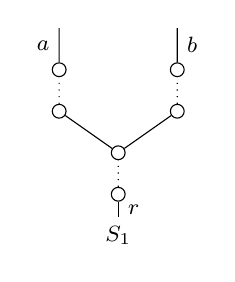
\begin{tikzpicture}
                  [grow=up,auto,
                  level distance=2em,
                  every node/.style = {font=\footnotesize,solid},
                  dummy/.style={circle,draw,inner sep=0pt,minimum size=1.75mm},
                  emph/.style={edge from parent/.style={black,thin,dotted,draw}},
                  norm/.style={edge from parent/.style={black,thin,draw,solid}}
                  ]
                  \node {$S_1$}
                  child[norm, level distance=1.5em] {node [dummy] {}
                    % child[norm, level distance=1.2em] {node [dummy] {}
                      child[emph]{node [dummy] {} % vertex
                        child[norm] {node [dummy] {}
                          child[emph] {node [dummy] {}
                            child[norm] {edge from parent node [swap] {$b$}}
                          }
                        }
                         child[norm] {node [dummy] {}
                          child[emph] {node [dummy] {}
                            child[norm] {edge from parent node {$a$}}
                          }
                        }
                      }
                      % }
                    edge from parent node [swap] {$r$}
                  };
            \end{tikzpicture}
      \]
      where there are $n_r$, $n_b$, and $n_a$ edges on the bottom, right, and left paths respectively.
\end{example}
      
Now, $\mathbb F^{\mathbf E(T)}\eta_{\mathbf E(T)}(\vect C) = \varnothing$ unless $\vect C = (e;e)$ for some $e \in \mathbf E(T)$;
in this case, $\mathbb F^{\mathbf E(T)}\eta(e;e) = \mathbb Z_{\geq 0}$, as in \eqref{FET_EE_EQ}.
% 
If we also denote the unit map by $\eta$, we see that the image of the map
\[
      \mathbb F^{\mathbf E(T)}\eta \xrightarrow{\mathbb F^{\mathbf E(T)}\eta} \mathbb F^{\mathbf E(T)} \Omega(T)
\]
corresponds to all factorizations from \eqref{FET_EQ} with $S_1$ a linear tree and $\phi$ (and hence $\psi_1$) a degeneracy.

Thus in the pushout $\mathbb F^{\mathbf E(T)}_\eta\Omega(T)$, all the non-injective operations are identified, and we have
\begin{align*}
  \mathbb F^{\mathbf E(T)}_\eta\Omega(T)(\vect C)
  & = \set{\mbox{factorizations $C \xrightarrow{\psi_0} S_1 \xrightarrow{\psi_1} T$ of $\phi$ with $\psi_1$ injective, $\psi_0$ tall}} \\
  & = \set{\mbox{inner faces $S_1$ of $T_{\phi(1 2 \dots n) \leq \phi(0)}$}} \\
  & = \set{\mbox{subsets $S_1 \subseteq \mathbf E^i(T_{\phi(1 2 \dots n) \leq \phi(0)})$ of inner edges}}    
\end{align*}
where $1 2 \dots n \leq 0$ is the vertex of $C$ and $T_{\phi(1 2 \dots n) \leq \phi(0)}$ is the associated outer face of $T$ \todo{find citation from \cite{Per18} /add discussion}.


% Iterating, we see that
% \[
%       \mathbb F(\mathbb F_\eta \Omega(T))(C)
%       = \set{
%         \begin{array}{l}
%           \mbox{factorizations $C \xrightarrow{\psi_0} S_1 \xrightarrow{\psi_1} S_2 \xrightarrow{\psi_2} T$}
%           \\
%           \mbox{of $\phi$ with $\psi_0,\psi_1$ tall and $\psi_2$ injective}
%         \end{array}
%       },
% \]
% while the image of $\eta$ in $\mathbb F_\eta \Omega(T)$ are those factorizations with
% $S_1 = \eta$,
% and the image of $\mathbb F(\eta)$ in $\mathbb F(\mathbb F_\eta \Omega(T)$ are those factorizations with
% $S_1$ linear and $S_2 = \eta$.

Inductively, we have the following:
\begin{align*}
  \left(\mathbb F^{\mathbf E(T)}_\eta \right)^{n-1} \Omega(T)(\vect C)
  & = \set{
    \begin{array}{l}
      \mbox{factorizations $C \xrightarrow{\ \quad \psi_0 \quad \ } S_1 \xrightarrow{\psi_1}
      % S_2 \xrightarrow{\psi_2}
      \dots \xrightarrow{\psi_{n-2}} S_{n-1} \xrightarrow{\psi_{n-1}} T$}
      \\
      \mbox{of $\phi$ with $\psi_i$ injective for $i > 0$ and $\psi_i$ tall for $i < n-1$}
    \end{array}
  },
  \\ % --------------------
  \mathbb F^{\mathbf E(T)} \left(\mathbb F^{\mathbf E(T)}_\eta\right)^{n-1} \Omega(T) (\vect C)
  & = \set{
    \begin{array}{l}
      \mbox{factorizations $C \xrightarrow{\psi_0} S_1 \xrightarrow{\psi_1} S_2 \xrightarrow{\psi_2} \dots \xrightarrow{\psi_{n-1}} S_n \xrightarrow{\psi_n} T$}
      \\
      \mbox{of $\phi$ with $\psi_i$ tall for $i < n$ and injective for $i > 1$}
    \end{array}
  },
  \\ % --------------------
  \mathsf{im}\left(\eta \to \left(\mathbb F^{\mathbf E(T)}_{\eta}\right)^{n-1}\Omega(T)\right)
  & = \set{
    \begin{array}{l}
      \mbox{factorizations $C_1 \xrightarrow{\ \quad \psi_0 \ \quad} \eta \xrightarrow{\psi_1}
        % \eta \xrightarrow{\psi_2}
      \dots \xrightarrow{\psi_{n-2}} \eta \xrightarrow{\psi_{n-1}} T$}
    \end{array}
  },
  \\ % --------------------
  \mathsf{im}\left(\mathbb F^{\mathbf E(T)}\left( \eta \to \left(\mathbb F^{\mathbf E(T)}_{\eta}\right)^n\Omega(T)\right)\right)
  & = \set{
    \begin{array}{l}
      \mbox{factorizations $C_1 \xrightarrow{\psi_0} S_1 \xrightarrow{\psi_1} \eta \xrightarrow{\psi_2} \dots \xrightarrow{\psi_{n-1}} \eta \xrightarrow{\psi_n} T$}
      \\
      \mbox{of $\phi$ with $S_1$ linear}
    \end{array}
  },
  \\ % --------------------
  \left(\mathbb F^{\mathbf E(T)}_\eta \right)^n \Omega(T)(\vect C)
  & = \set{
    \begin{array}{l}
      \mbox{factorizations $C \xrightarrow{\psi_0} S_1 \xrightarrow{\psi_1} S_2 \xrightarrow{\psi_2} \dots \xrightarrow{\psi_{n-1}} S_n \xrightarrow{\psi_n} T$}
      \\
      \mbox{of $\phi$ with $\psi_i$ injective for $i > 0$ and $\psi_i$ tall for $i < n$}
    \end{array}
  }
  \\
  &= \set{\mbox{nested subsets $S_1 \subseteq S_2 \subseteq \dots \subseteq S_n \subseteq \mathbf E^i(T_{\phi(1 2 \dots n) \leq \phi(0)})$}}.
  % \\
  % \left(\mathbb F^{\mathbf E(T)}\right)^n \Omega(T)(\vect C)
  % & = \set{
  %   \begin{array}{l}
  %     \mbox{factorizations $C \xrightarrow{\psi_0} S_1 \xrightarrow{\psi_1} S_2 \xrightarrow{\psi_2} \dots \xrightarrow{\psi_{n-1}} S_n \xrightarrow{\psi_n} T$}
  %     \\
  %     \mbox{of $\phi$ with $\psi_i$ tall for $i < n$}
  %   \end{array}
  % }
\end{align*}

Finally, for any finite set $A$, we recall that the $n$-simplicies of $\Delta[1]^{\times A}$ correspond to $(n+1)$-strings of nested subsets of $A$.
Thus we have the following description of $W(T)$:

\begin{equation}
      \label{WT_EQ}
      W(T)(\vect C) = 
      \begin{cases}
            \Delta[1]^{\times \mathbf E^i(T_{\underline e \leq e})}, \qquad & \mbox{there exist $C \xrightarrow{\phi} T$ with $\partial \phi = \vect C$}
            \\
            \varnothing & \text{else,}
      \end{cases}
\end{equation}

It is clear that $W(-)$ is functorial. Thus we have the following definition.








\bibliography{biblio3}{}
\bibliographystyle{amsalpha2}



\end{document}

